\documentclass[12pt,a4paper,oneside]{article}

\usepackage{fontspec}
\IfFontExistsTF{TeX Gyre Termes}{\setmainfont{TeX Gyre Termes}}{\setmainfont{Times New Roman}}
\IfFontExistsTF{TeX Gyre Cursor}{\setmonofont[Scale=0.86]{TeX Gyre Cursor}}{\setmonofont[Scale=0.84]{Consolas}}

\usepackage[top=2.5cm,bottom=2.5cm,left=2.54cm,right=2.54cm,headheight=28pt,headsep=16pt,footskip=24pt]{geometry}
\usepackage{graphicx}
\usepackage{booktabs}
\usepackage{tabularx}
\usepackage{array}
\usepackage{amsmath}
\usepackage{amssymb}
\usepackage{xcolor}
\usepackage{fancyhdr}
\usepackage{lastpage}
\usepackage[font=small,labelfont=bf,skip=6pt]{caption}
\usepackage{float}
\usepackage[section]{placeins}
\usepackage{enumitem}
\usepackage{setspace}
\usepackage{tikz}
\usetikzlibrary{arrows.meta,positioning}
\usepackage[hidelinks,breaklinks=true,plainpages=false,pdfpagelabels]{hyperref}

\setcounter{tocdepth}{2}

\definecolor{hcmutblue}{RGB}{0,51,153}
\definecolor{hcmutcyan}{RGB}{0,130,214}
\definecolor{softbg}{RGB}{244,247,252}

\urlstyle{same}
\setstretch{1.2}
\setlength{\parindent}{1.5em}
\setlength{\parskip}{0.35em}
\setlength{\emergencystretch}{2.5em}
\setlist[itemize]{topsep=4pt,itemsep=3pt,parsep=0pt}
\setlist[enumerate]{topsep=4pt,itemsep=3pt,parsep=0pt}

\newcolumntype{L}[1]{>{\raggedright\arraybackslash}p{#1}}
\newcolumntype{C}[1]{>{\centering\arraybackslash}p{#1}}
\newcolumntype{R}[1]{>{\raggedleft\arraybackslash}p{#1}}
\newcolumntype{Y}{>{\raggedright\arraybackslash}X}

\fancypagestyle{hcmutbody}{
  \fancyhf{}
  \fancyhead[L]{
\includegraphics[height=0.58cm]{figures/hcmut_logo.png}\hspace{5pt}\raisebox{0.14cm}{\small HCMUT}}
  \fancyhead[R]{\raisebox{0.14cm}{\small P4AI-DS (CO3135) --- Course Project Report}}
  \fancyfoot[R]{\small Page \thepage\ of \pageref{LastPage}}
  \renewcommand{\headrulewidth}{0.4pt}
  \renewcommand{\footrulewidth}{0.4pt}
}

\fancypagestyle{plain}{
  \fancyhf{}
  \fancyfoot[C]{\small \thepage}
  \renewcommand{\headrulewidth}{0pt}
  \renewcommand{\footrulewidth}{0pt}
}

\begin{document}

% ==============================================================================
% COVER PAGE (HCMUT CSE Standard)
% ==============================================================================
\begin{titlepage}
  \thispagestyle{empty}
  \centering
  {\large\bfseries VIETNAM NATIONAL UNIVERSITY HO CHI MINH CITY\par}
  \vspace{4pt}
  {\large\bfseries HO CHI MINH CITY UNIVERSITY OF TECHNOLOGY\par}
  \vspace{4pt}
  {\normalsize\bfseries FACULTY OF COMPUTER SCIENCE AND ENGINEERING\par}
  \vspace{6pt}
  \rule{0.25\textwidth}{0.6pt}\par

  \vspace{1.2cm}
  
\includegraphics[width=3.8cm]{figures/hcmut_logo.png}\par
  \vspace{1.2cm}

  \rule{\textwidth}{0.8pt}\par
  \vspace{12pt}
  {\Large\bfseries COURSE PROJECT REPORT\par}
  \vspace{10pt}
  \rule{\textwidth}{0.8pt}\par

  \vspace{0.9cm}
  {\large\bfseries Programming for Artificial Intelligence and Data Science (CO3135)\par}
  \vspace{4pt}
  {\normalsize Class: \texttt{CLC\_HK261 [CC01]}\par}
  \vspace{16pt}
  {\LARGE\bfseries Vehicle Loan Default Prediction:\\An Empirical Machine Learning Study\par}

  \vspace{1.5cm}
  {\normalsize \textbf{Lecturer:} \quad Trần Huy\par}
  \vspace{0.9cm}

  \begin{tabular}{||l|c||}
    \hline\hline
    \multicolumn{1}{||c|}{\textbf{Student Name}} & \textbf{Student ID} \\
    \hline\hline
    Dương Đăng Khoa & 2352551 \\
    \hline\hline
  \end{tabular}

  \vfill
  {\normalsize Ho Chi Minh City, November 2026\par}
\end{titlepage}

% ==============================================================================
% FRONT MATTER: ABSTRACT, TOC, LIST OF FIGURES & LIST OF TABLES (Roman Pages)
% ==============================================================================
\pagenumbering{roman}
\pagestyle{plain}

\section*{Abstract}
\addcontentsline{toc}{section}{Abstract}
Predicting First Payment Default (FPD) in emerging-market vehicle financing is challenging because over half of applicants lack a numerical credit bureau score ($55.66\%$), default prevalence shifts sharply over time, and misclassification costs are strongly asymmetric. This project designs and evaluates an end-to-end, leakage-free machine learning pipeline on $233{,}154$ labeled L\&T Financial Services (LTFS) vehicle loan contracts disbursed between August and October 2018. Using a date-clean Out-of-Time (OOT) split (Development $N = 182{,}501$ through October 22, default rate $20.63\%$; Locked OOT Test $N = 50{,}653$ from October 23--31, default rate $25.59\%$), we benchmark six models spanning linear, tree-based, gradient-boosted, and neural paradigms (\texttt{LogisticRegression}, \texttt{DecisionTree}, \texttt{RandomForest}, \texttt{XGBoost}, \texttt{LightGBM}, and \texttt{MLP}) across four nested feature-engineering tiers, fold-isolated Out-of-Fold Empirical-Bayes target encoding, Optuna hyperparameter optimization, six class-imbalance treatments, cost-sensitive decision thresholding, and TreeSHAP explainability. On the Locked OOT Test cohort, tuned \texttt{LightGBM} ($\text{ROC-AUC} = 0.6621$, $\text{PR-AUC} = 0.3910$) and \texttt{XGBoost} ($\text{ROC-AUC} = 0.6620$, $\text{PR-AUC} = 0.3907$) lead all models, clearly outperforming \texttt{RandomForest} ($0.6554$), \texttt{LogisticRegression} ($0.6525$), the \texttt{MLP} baseline ($0.6525$), and \texttt{DecisionTree} ($0.6270$). Comparative testing reveals that standard 80/20 random splitting inflates ROC-AUC by $+0.0091$ to $+0.0106$ and hides a $30$-fold increase in calibration error ($\text{ECE } 0.0016 \to 0.0491$) under temporal prior shift. Finally, fold-isolated \texttt{SMOTE} degrades \texttt{LightGBM} OOT ROC-AUC to $0.6252$, whereas retaining natural class priors with a Bayesian $5{:}1$ cost threshold ($\tau = 0.167$) reduces principal-weighted portfolio loss from $13.12\%$ (at $\tau = 0.50$) to $7.13\%$ while maintaining stable TreeSHAP attributions ($\rho = 0.973$ from Development to OOT Test).
\clearpage

\tableofcontents
\clearpage
\listoffigures
\addcontentsline{toc}{section}{List of Figures}
\vspace{1em}
\listoftables
\addcontentsline{toc}{section}{List of Tables}
\clearpage

% ==============================================================================
% MAIN BODY (Arabic Page Numbers)
% ==============================================================================
\pagenumbering{arabic}
\pagestyle{hcmutbody}

\section{Problem Definition and Dataset Overview}
\label{sec:problem_data}

\subsection{Problem Statement and Motivation}
In emerging-market vehicle financing, lenders extend loans for motorcycles and light commercial vehicles to many first-time borrowers who lack an established credit history. A key risk indicator in this setting is \textbf{First Payment Default (FPD)}, defined as a borrower failing to pay the very first scheduled monthly installment on time. Early default directly reflects immediate repayment difficulty, weak point-of-sale screening, or dealer-level adverse selection, making pre-disbursal risk prediction essential before loan approval.

We formulate vehicle loan default prediction as a supervised binary classification and probability estimation problem. Given pre-disbursal borrower demographics, loan contract terms, dealer and regional attributes, and prior credit-bureau records $\mathbf{x}_i$, the goal is to estimate the probability $\hat{p}_i = P(y_i = 1 \mid \mathbf{x}_i)$ that an approved loan $i$ defaults on its first installment ($y_i = 1$). Because only pre-origination fields are observed at decision time, the pipeline must strictly exclude post-disbursal information and guard against data leakage.

Three real-world characteristics make this task challenging:
\begin{enumerate}
  \item \textbf{Prevalence of thin-file borrowers:} Over half of applicants ($55.66\%$) lack a numerical credit score, carrying special status codes ($<300$) rather than continuous scores ($300\text{--}890$).
  \item \textbf{Moderate class imbalance with asymmetric error costs:} Roughly $21.71\%$ of approved contracts default ($3.61{:}1$ negative-to-positive ratio). Missing an actual default sacrifices substantial loan principal, whereas falsely flagging a reliable borrower causes only a smaller opportunity cost or manual review expense.
  \item \textbf{Temporal shift across origination cohorts:} Application volumes and default rates fluctuate markedly across weeks and festive seasons, so models trained on past months must generalize to future contracts rather than randomly sampled dates.
\end{enumerate}

\subsection{Dataset Overview and Exploratory Findings}
This project uses the L\&T Financial Services (LTFS) Vehicle Loan Default Prediction dataset~\cite{ltfs2019}, containing $233{,}154$ labeled contracts disbursed over $84$ active days from August 1 to October 31, 2018 ($41$ raw columns), alongside an unlabeled competition test file of $112{,}392$ contracts from November 2018. Although the November file cannot be scored without labels, its future timestamp confirms that real deployment operates sequentially over time. Table~\ref{tab:dataset_summary} summarizes our automated audit of the labeled dataset prior to modeling.

\begin{table}[htbp]
  \centering
  \caption{Summary profile and data-integrity audit of the labeled LTFS dataset ($N = 233{,}154$).}
  \label{tab:dataset_summary}
  \footnotesize
  \begin{tabularx}{\textwidth}{@{}L{3.8cm} Y@{}}
    \toprule
    \textbf{Property} & \textbf{Verified Observation and Cleaning Action} \\
    \midrule
    Dataset size & $233{,}154$ labeled rows $\times$ $41$ columns ($0$ duplicate contracts). \\
    Target (\texttt{loan\_default}) & $50{,}611$ defaults ($21.71\%$) vs.\ $182{,}543$ non-defaults ($78.29\%$); ratio $3.61{:}1$. \\
    Dropped columns & Dropped \texttt{UniqueID} (monotonically ordered by date, Spearman $\rho = 0.9998$, causing severe time leakage) and \texttt{MobileNo\_Avl\_Flag} (constant value $1$). \\
    Birth-year century fix & $19{,}866$ records ($8.52\%$) had two-digit birth years (\texttt{'00}--\texttt{'68}) misparsed as $20\text{xx}$; normalized to valid borrower ages in $[18.0, 69.1]$ years. \\
    Missing values & Only \texttt{Employment.Type} had missing entries ($3.29\%$); preserved as explicit \texttt{"MISSING"} category because employment categories differ significantly in default rate ($\chi^2\ p = 3.12 \times 10^{-42}$) and missingness varies non-randomly across states ($\chi^2\ p < 10^{-100}$), though binary missing vs.\ non-missing default rates are similar ($p = 0.60$). \\
    Credit bureau scale & $55.66\%$ carry non-scored codes ($<300$); $44.34\%$ hold scores in $300\text{--}890$. \\
    Heavy right skew & Bureau balances, limits, and installments contain $60.5\%\text{--}99.4\%$ zeros with extreme upper-tail skewness ($29.4$ for \texttt{PRI.CURRENT.BALANCE}, $69.9$ for \texttt{PRIMARY.INSTAL.AMT}, up to $323.7$ for \texttt{PRI.SANCTIONED.AMOUNT}); \texttt{ltv} median is $76.8\%$ (capped at $95.0\%$). \\
    High-cardinality channels & \texttt{Current\_pincode\_ID} ($6{,}698$ levels), \texttt{Employee\_code\_ID} ($3{,}270$), \texttt{supplier\_id} ($2{,}953$), and \texttt{branch\_id} ($82$). \\
    \bottomrule
  \end{tabularx}
\end{table}

Univariate screening across all raw attributes confirmed no target leakage in individual features (highest single-feature ROC-AUC $\le 0.569$ for \texttt{ltv}), and bureau records almost never match the new vehicle loan ($0.0013\%$ overlap), verifying that credit histories strictly precede the current application.

To prevent any exploratory bias from leaking into test evaluation, all distribution plots were generated solely on the Development partition (\texttt{2018-08-01} to \texttt{2018-10-22}, $N = 182{,}501$, default rate $20.63\%$), keeping the late-October test window (\texttt{2018-10-23} to \texttt{2018-10-31}, $N = 50{,}653$, $25.59\%$ default rate) sealed. Figure~\ref{fig:eda_target} highlights clear temporal non-stationarity: monthly portfolio default rates shift from $21.57\%$ in August ($68{,}002$ loans) down to $19.19\%$ in September ($66{,}788$ loans) before rising to $23.51\%$ across October ($98{,}364$ loans) and jumping to $25.59\%$ during the final festival-week wave (peaking at $29.65\%$ on October 31).

\begin{figure}[htbp]
  \centering
  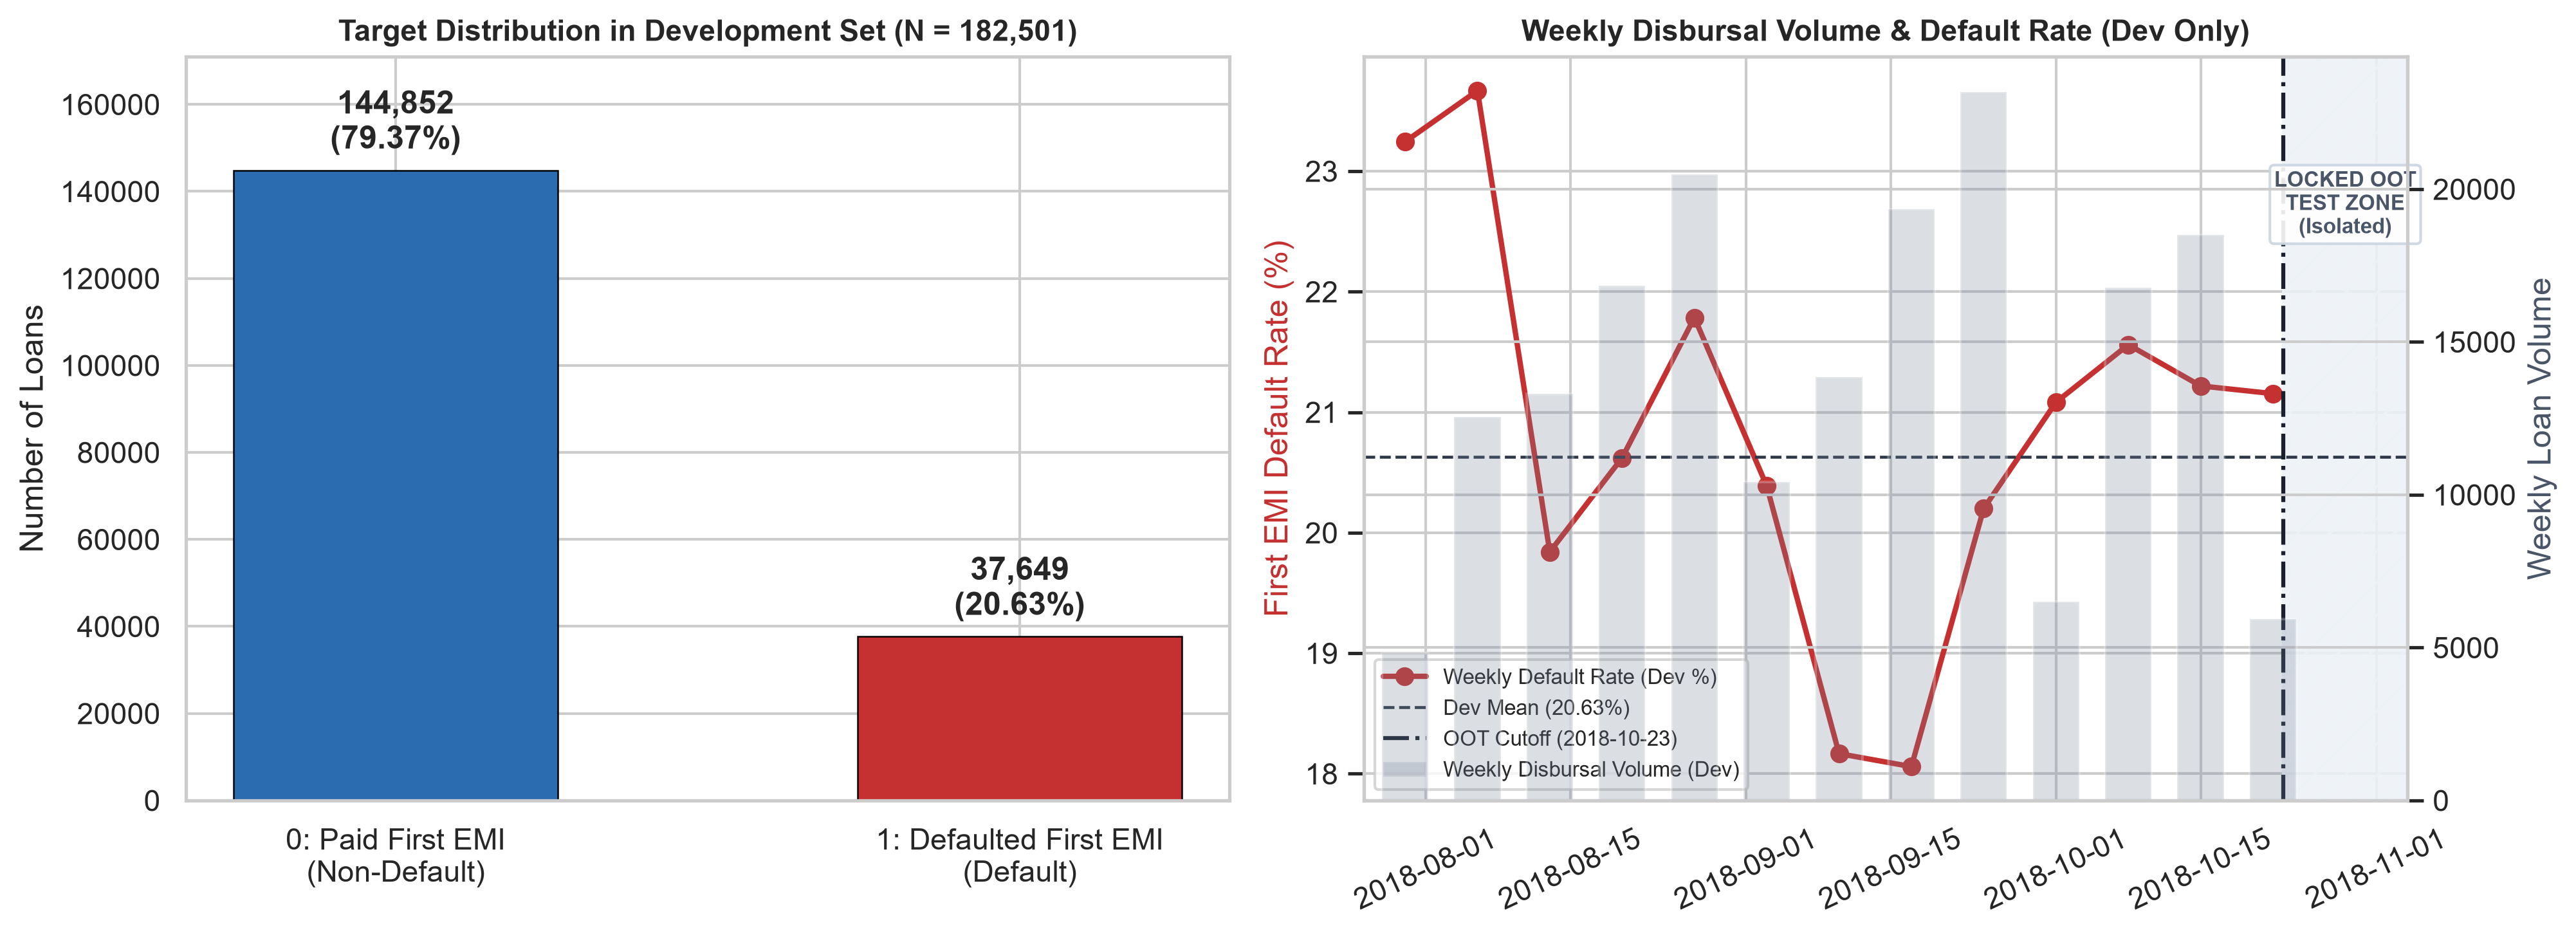
\includegraphics[width=0.95\textwidth]{figures/eda_01_target_and_splits.png}
  \caption{Development-set target distribution ($N = 182{,}501$, left) and weekly loan volume alongside default rate drift up to the October 23 Out-of-Time cutoff (right).}
  \label{fig:eda_target}
\end{figure}

Figure~\ref{fig:eda_bureau} demonstrates why the raw \texttt{PERFORM\_CNS.SCORE} field cannot be treated as a single continuous number. More than half of borrowers hold special status codes below $300$, whose default risk varies by reason code---from $17.6\%$ in Development ($18.6\%$ full corpus) for stale/inactive histories up to $24.1\%$ Dev ($25.6\%$ full corpus) for insufficient-history flags. Conversely, among scored borrowers ($300\text{--}890$), default risk exhibits a broadly upward trend across alphabetical risk grades \texttt{A}--\texttt{M}---rising from $12.0\%\text{--}16.5\%$ in Development ($13.1\%\text{--}17.3\%$ full corpus) for tiers \texttt{A}--\texttt{D} to $29.3\%$ Dev ($30.5\%$ full corpus) in tier \texttt{M}, with minor local inversions at grades \texttt{B}, \texttt{D}, and \texttt{J}.

\begin{figure}[htbp]
  \centering
  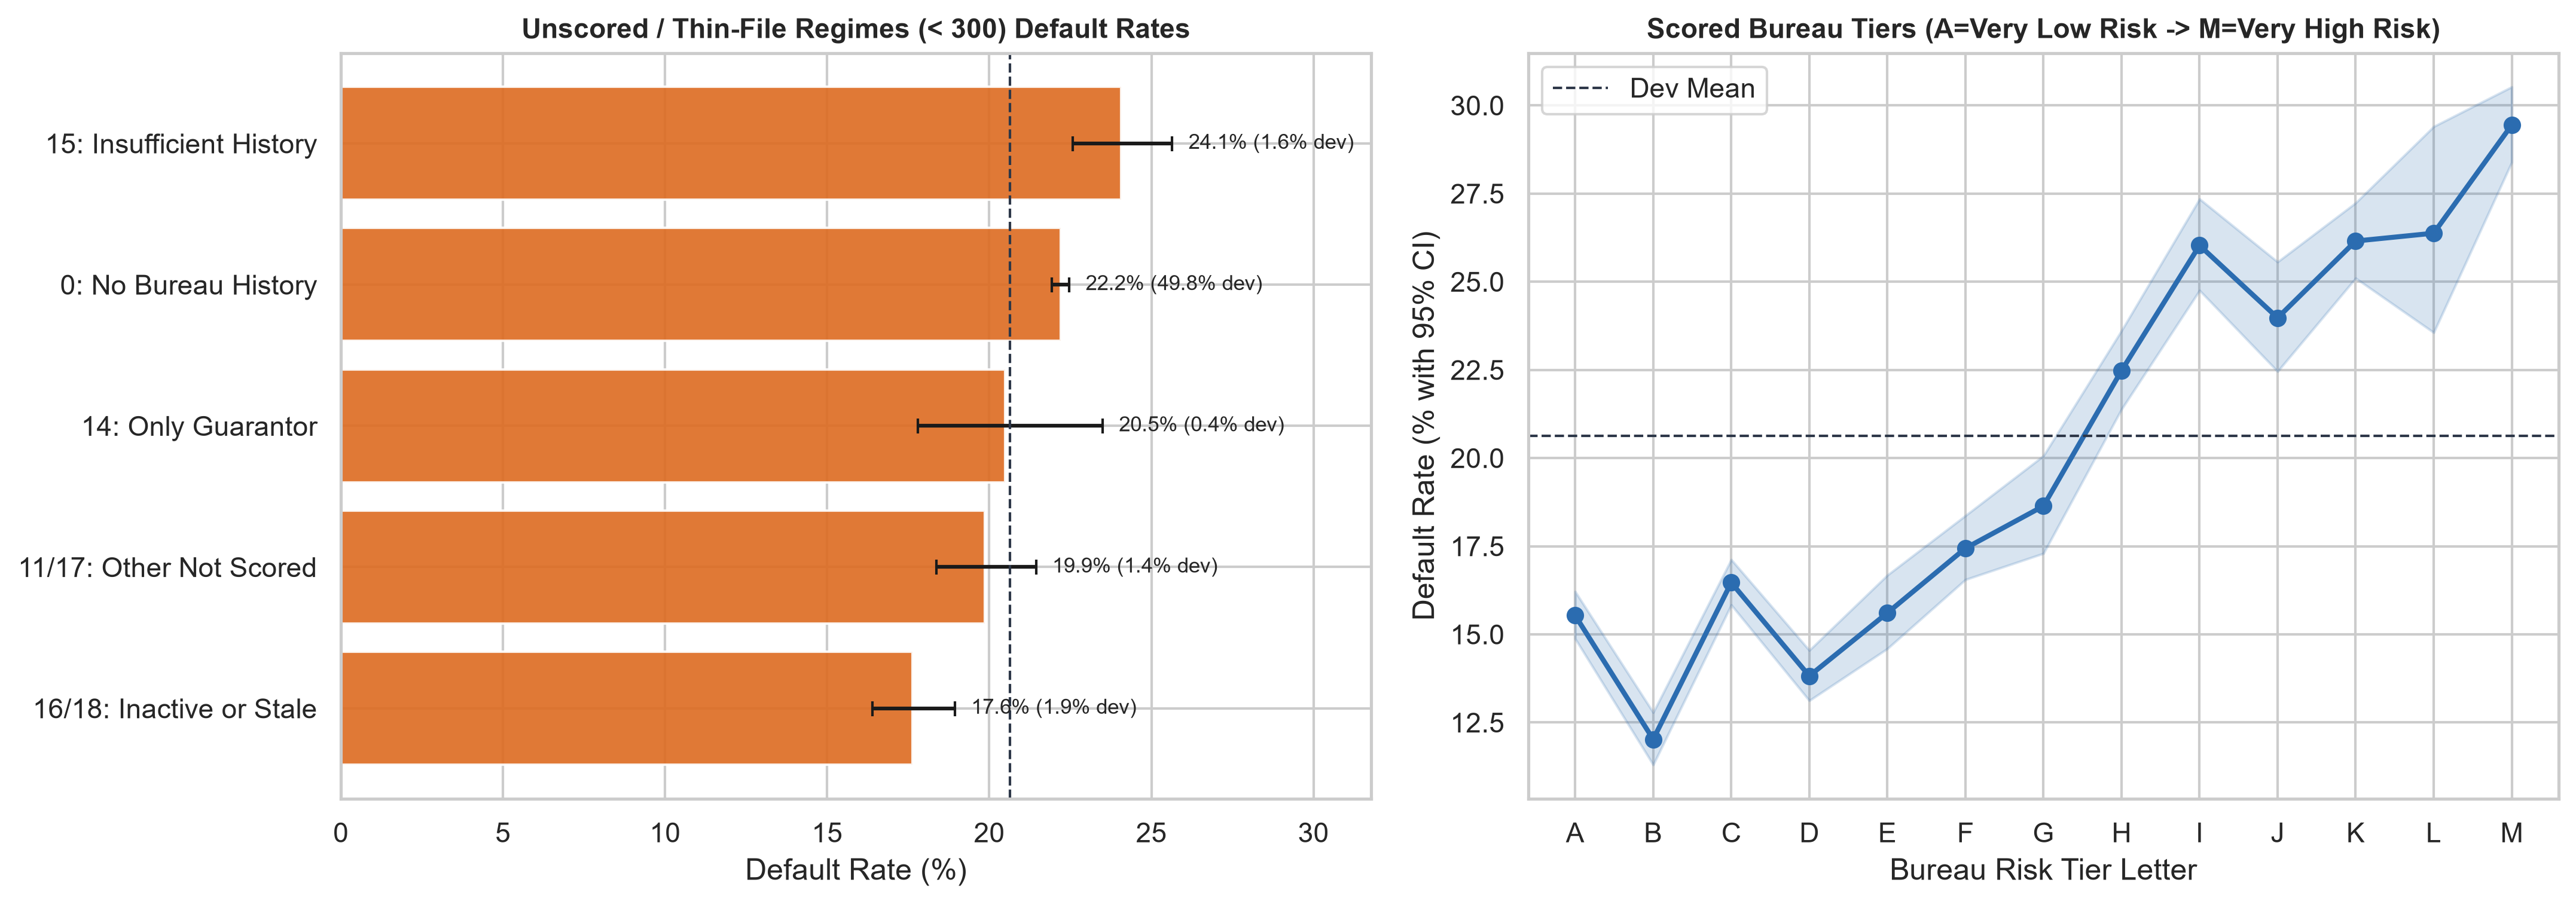
\includegraphics[width=0.95\textwidth]{figures/eda_04_bureau_regime_and_score_risk.png}
  \caption{Dual-regime credit bureau risk in the Development Set ($N = 182{,}501$): non-scored thin-file codes ($<300$, left) versus broad upward risk progression across scored tiers \texttt{A}--\texttt{M} (right).}
  \label{fig:eda_bureau}
\end{figure}

Further exploratory checks revealed three additional signals that guided feature design: (i) loan-to-value leverage (\texttt{ltv}) strongly stratifies default risk, nearly doubling from $13.1\%$ in the lowest decile to $25.8\%$ in the highest decile (and exceeding $29\%$ for high-LTV thin-file loans); (ii) \texttt{Self employed} borrowers default more frequently ($21.7\%$ on Dev) than \texttt{Salaried} ($19.4\%$) or missing-employment records ($20.0\%$); and (iii) ledger inconsistencies contain predictive risk signals, such as borrowers whose overdue accounts exceed active accounts ($27.5\%$ full-corpus default), current balances exceeding sanctioned limits ($24.3\%$), negative primary credit balances ($14.5\%$; $14.1\%$ combined primary/secondary), or gaps $>5$ percentage points between declared and computed LTV ($3.5\%$ of contracts).

\section{Literature Review}
\label{sec:literature}

\subsection{Credit Scoring: Classical Models, Gradient Boosting, and Deep Learning}
Financial and credit-scoring studies consistently identify borrower credit bureau ratings, loan-to-value (LTV) leverage, vehicle attributes, and lending-channel heterogeneity as core determinants of auto loan default~\cite{agarwal2008}. In traditional retail credit benchmarks, Baesens et al.~\cite{baesens2003} showed that well-regularized Logistic Regression (LR) provides a transparent and competitive baseline relative to single decision trees and early neural networks. Updating these benchmarks across diverse credit portfolios, Lessmann et al.~\cite{lessmann2015} demonstrated that tree ensembles---specifically Random Forests~\cite{breiman2001} and Gradient Boosting---outperform standalone linear and tree classifiers with statistical significance, while emphasizing that incremental AUC gains should always be weighed against interpretability and operational cost.

On structured tabular datasets, Gradient Boosted Decision Tree (GBDT) frameworks lead modern practice, notably \textbf{XGBoost}~\cite{chen2016} (regularized second-order boosting with sparsity-aware branching for missing values and dense zeros) and \textbf{LightGBM}~\cite{ke2017} (fast histogram-based leaf-wise tree growth). Whether deep neural networks surpass GBDTs on consumer credit tables remains widely studied. Both Gunnarsson et al.~\cite{gunnarsson2021} and Grinsztajn et al.~\cite{grinsztajn2022} concluded across large empirical benchmarks that GBDTs match or outperform Multilayer Perceptrons (MLPs) and tabular deep networks at much lower tuning cost, because axis-aligned tree splits naturally model sharp thresholds and resist uninformative features. Notably, a recent paper on the LTFS dataset by Wu~\cite{wu2025} reported an unusually large jump from LR ($\text{AUC}=0.62$) to XGBoost with SMOTE ($\text{AUC}=0.89$), yet relied on random train-test splitting without temporal validation, calibration auditing, or fold-isolated resampling controls.

\subsection{Class Imbalance, Calibration, and Cost-Sensitive Decisions}
While oversampling methods such as SMOTE~\cite{chawla2002} are frequently applied by default to imbalanced data, empirical risk-modeling evidence cautions against uncritical resampling. van den Goorbergh et al.~\cite{goorbergh2022} proved that random undersampling and SMOTE do not improve ROC-AUC separation on moderately imbalanced risk data while severely distorting predicted probabilities (ruining calibration). Furthermore, Saito and Rehmsmeier~\cite{saito2015} demonstrated that Precision--Recall curves (PR-AUC) are more informative than ROC curves alone under class imbalance. Decision theory establishes that when a model predicts well-calibrated risk scores on the natural class prior, asymmetric financial trade-offs should be handled through the Bayes-optimal threshold $c_{\text{FP}}/(c_{\text{FP}}+c_{\text{FN}})$~\cite{elkan2001} or principal-weighted loan cost metrics~\cite{bahnsen2014} rather than synthetic data generation.

\subsection{Explainable AI in Credit Risk}
Because consumer lending requires transparent adverse-action explanations, model interpretability is essential alongside predictive accuracy. Building on the game-theoretic SHAP framework~\cite{lundberg2017}, Lundberg et al.~\cite{lundberg2020} introduced \textbf{TreeSHAP} to compute exact Shapley feature attributions and pairwise interactions for tree ensembles, resolving the inconsistency of traditional split-gain counts while cautioning that strongly correlated predictors share credit across tree splits. Extending SHAP to credit governance, Bussmann et al.~\cite{bussmann2021} showed how Shapley auditing and subgroup analysis uncover distinct borrower risk profiles and highlight fairness risks.

Table~\ref{tab:lit_summary} summarizes the main literature themes and how they directly inform our project pipeline.

\begin{table}[htbp]
  \centering
  \caption{Summary of key literature themes and direct implications for our LTFS pipeline.}
  \label{tab:lit_summary}
  \footnotesize
  \begin{tabularx}{\textwidth}{@{}L{3.4cm} L{2.8cm} Y Y@{}}
    \toprule
    \textbf{Theme} & \textbf{Key References} & \textbf{Established Findings} & \textbf{Design Decision Here} \\
    \midrule
    Auto loans \& tabular model choice & \cite{agarwal2008,baesens2003,lessmann2015,gunnarsson2021,grinsztajn2022} & Credit score, LTV, and dealer channels drive risk; GBDTs outperform LR and tabular MLPs with lower compute. & Benchmark LR, DT, RF, XGBoost, LightGBM, and MLP under clean features and OOT testing. \\[3pt]
    GBDT categoricals \& LTFS gaps & \cite{chen2016,ke2017,wu2025,miccibarreca2001} & Zero-inflated tables suit GBDTs; naive target encoding or random splits cause optimism bias. & Use Out-of-Time validation and strict Out-of-Fold Empirical-Bayes target encoding on high-cardinality IDs. \\[3pt]
    Imbalance, calibration \& cost scoring & \cite{chawla2002,goorbergh2022,saito2015,elkan2001,bahnsen2014} & Resampling skews probability calibration without lifting AUC; PR-AUC and cost-based cutoffs reflect risk better. & Compare fold-isolated SMOTE, RUS, and class weights vs.\ natural prior with Bayesian and principal-weighted thresholds. \\[3pt]
    Credit explainability & \cite{lundberg2017,lundberg2020,bussmann2021} & TreeSHAP gives exact local/global explanations; collinear features share attribution. & Apply exact TreeSHAP with Dev-to-OOT stability checks, error cases, and thin-file audits. \\
    \bottomrule
  \end{tabularx}
\end{table}

\section{Methodology and Algorithm Implementation}
\label{sec:methodology}

\subsection{Pipeline Overview and Data-Splitting Strategy}
To guarantee reproducible, leakage-free comparisons, the entire workflow operates under a unified random seed ($\text{seed} = 42$) and strict partition isolation. All preprocessing statistics, target encodings, hyperparameter searches, calibration curves, and operating cutoffs are derived exclusively from the Development set and frozen prior to single-pass evaluation on the unseen Test set. Figure~\ref{fig:pipeline} illustrates the six-stage pipeline.

\begin{figure}[htbp]
  \centering
  \resizebox{\textwidth}{!}{%
  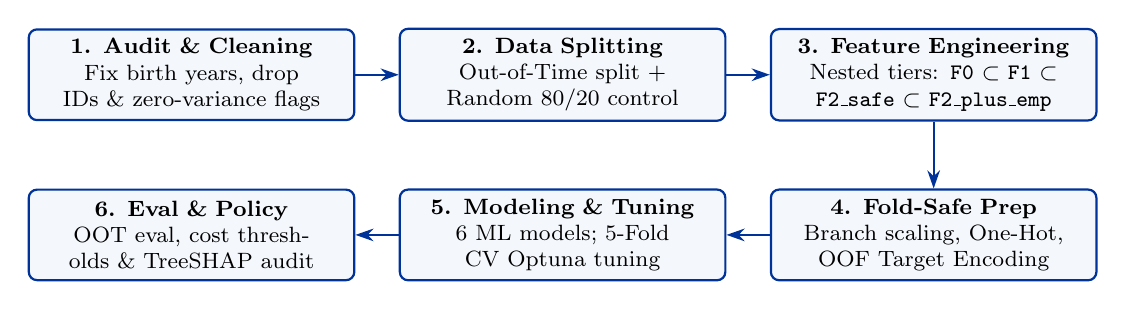
\begin{tikzpicture}[
    node distance=0.45cm and 0.55cm,
    box/.style={
      rectangle, rounded corners=3pt, draw=hcmutblue, fill=softbg,
      thick, align=center, font=\footnotesize, minimum height=1.15cm, text width=3.9cm
    },
    arrow/.style={-{Stealth[length=2.3mm,width=1.6mm]}, thick, color=hcmutblue}
  ]
    \node[box] (s1) {\textbf{1. Audit \& Cleaning}\\Fix birth years, drop IDs \& zero-variance flags};
    \node[box, right=of s1] (s2) {\textbf{2. Data Splitting}\\Out-of-Time split + Random 80/20 control};
    \node[box, right=of s2] (s3) {\textbf{3. Feature Engineering}\\Nested tiers: \texttt{F0} $\subset$ \texttt{F1} $\subset$ \texttt{F2\_safe} $\subset$ \texttt{F2\_plus\_emp}};
    \node[box, below=0.85cm of s3] (s4) {\textbf{4. Fold-Safe Prep}\\Branch scaling, One-Hot, OOF Target Encoding};
    \node[box, left=of s4] (s5) {\textbf{5. Modeling \& Tuning}\\6 ML models; 5-Fold CV Optuna tuning};
    \node[box, left=of s5] (s6) {\textbf{6. Eval \& Policy}\\OOT eval, cost thresholds \& TreeSHAP audit};

    \draw[arrow] (s1) -- (s2);
    \draw[arrow] (s2) -- (s3);
    \draw[arrow] (s3) -- (s4);
    \draw[arrow] (s4) -- (s5);
    \draw[arrow] (s5) -- (s6);
  \end{tikzpicture}%
  }
  \caption{End-to-end leakage-free machine learning pipeline built for vehicle loan FPD prediction.}
  \label{fig:pipeline}
\end{figure}

Because real lending models score future applications based on past contracts, our primary evaluation uses a \textbf{Date-Clean Out-of-Time (OOT) Split} with a cutoff on \texttt{2018-10-23} (no calendar day is shared across Development and Test). Inside the Development partition ($N = 182{,}501$), 5-fold stratified cross-validation guides tuning and threshold selection. For direct comparison, we also build a \textbf{Stratified Random 80/20 Split} sampled uniformly across all dates to quantify how much random splitting overstates future performance. Table~\ref{tab:splits} summarizes both protocols.

\begin{table}[htbp]
  \centering
  \caption{Summary of the Primary Out-of-Time (OOT) and Comparative Stratified Random splits.}
  \label{tab:splits}
  \footnotesize
  \setlength{\tabcolsep}{3.5pt}
  \begin{tabular}{@{}llrrrc@{}}
    \toprule
    \textbf{Protocol} & \textbf{Partition} & \textbf{Contracts ($N$)} & \textbf{Defaults} & \textbf{Default Rate} & \textbf{Date Range} \\
    \midrule
    Primary OOT & Development (5-Fold CV) & $182{,}501$ & $37{,}649$ & $20.63\%$ & \texttt{2018-08-01}--\texttt{2018-10-22} \\
    (Main Study) & Locked OOT Test & $50{,}653$ & $12{,}962$ & $25.59\%$ & \texttt{2018-10-23}--\texttt{2018-10-31} \\
    \midrule
    Random 80/20 & Development (5-Fold CV) & $186{,}523$ & $40{,}489$ & $21.71\%$ & \texttt{2018-08-01}--\texttt{2018-10-31} \\
    (Control) & Locked Random Test & $46{,}631$ & $10{,}122$ & $21.71\%$ & \texttt{2018-08-01}--\texttt{2018-10-31} \\
    \bottomrule
  \end{tabular}
\end{table}

\subsection{Preprocessing and Feature Engineering}
All stateful preprocessing steps are wrapped inside \texttt{scikit-learn} pipelines fitted strictly on training folds during cross-validation, and on the full Development set prior to final OOT scoring. Because linear/neural models and tree ensembles treat feature scales differently, two tailored preprocessing branches are constructed:
\begin{itemize}
  \item \textbf{Linear and Neural Branch (LR, MLP):} Numerical ledger features are median-imputed (with missingness indicators), clipped at training $[0.5\%, 99.5\%]$ quantiles, compressed via $\operatorname{sign}(x)\ln(1+|x|)$ to stabilize heavy tails and negative balances, and standardized via \texttt{RobustScaler}/\texttt{StandardScaler}. Low-cardinality categoricals are one-hot encoded, and near-duplicate disbursed-amount fields ($\rho > 0.995$ with sanctioned amounts) are removed.
  \item \textbf{Tree Branch (DecisionTree, RandomForest, XGBoost, LightGBM):} Numerical attributes preserve their natural scales with median imputation and one-hot encoding for low-cardinality categories, allowing trees to split cleanly on raw rupee and percentage thresholds.
\end{itemize}

To utilize high-cardinality dealer, branch, and postal identifiers (\texttt{branch\_id}, \texttt{supplier\_id}, and \texttt{Current\_pincode\_ID}) without memorizing rare categories or leaking target labels, we pair training-fold category frequencies with an \textbf{Out-of-Fold Empirical-Bayes Target Encoder}~\cite{miccibarreca2001} ($K=5$ inner folds, smoothing parameter $m=50$):
\begin{equation}
\label{eq:oof_te}
  \hat{e}_{c}^{(k)} = \frac{\sum_{i \in \mathcal{D}_{-k} : x_i = c} y_i + m \cdot \bar{y}_{-k}}{n_{c,-k} + m},
\end{equation}
where $\bar{y}_{-k}$ is the out-of-fold default rate. During inference, categories unseen in training safely receive the global training prior $\bar{y}_{\text{train}}$ and frequency $0.0$.

To measure the value of domain feature engineering systematically, four nested feature tiers are constructed in Table~\ref{tab:features}. Notice that \texttt{Employee\_code\_ID} is isolated into Tier \texttt{F2\_plus\_emp} solely as an ablation test against personnel turnover and cold-start risk, leaving \texttt{F2\_safe} as our governed production feature set.

\begin{table}[htbp]
  \centering
  \caption{Four-tier nested feature engineering hierarchy and processed matrix dimensions.}
  \label{tab:features}
  \footnotesize
  \begin{tabularx}{\textwidth}{@{}llL{3.0cm}Y@{}}
    \toprule
    \textbf{Tier} & \textbf{Linear / Tree Cols} & \textbf{Scope} & \textbf{Engineered Signals Added} \\
    \midrule
    \texttt{F0} & $82$ / $84$ & Clean baseline & Drops IDs/constants; preserves missing employment; parses 3 duration/age fields (\texttt{age\_at\_disbursal}, \texttt{avg\_acct\_age\_months}, \texttt{credit\_history\_months}). \\[3pt]
    \texttt{F1} & $114$ / $117$ & $+29$ domain features & Separates bureau score $<300$ vs.\ $\ge 300$ (4 features); adds down-payment \& LTV discrepancy (4); sums primary + secondary credit totals \& KYC count (9); computes delinquency/utilization/inquiry ratios (7); adds ledger anomaly \& \texttt{ltv\_x\_no\_bureau} flags (5). \\[3pt]
    \texttt{F2\_safe} & $120$ / $123$ & $+$ Channel/Geo IDs & Adds OOF Target Encoding (Eq.~\eqref{eq:oof_te}) + frequency encoding for \texttt{branch\_id}, \texttt{supplier\_id}, and \texttt{Current\_pincode\_ID}. \\[3pt]
    \texttt{F2\_plus\_emp} & $122$ / $125$ & $+$ Officer ID & Adds \texttt{Employee\_code\_ID} ($3{,}270$ levels) to test cold-start sensitivity. \\
    \bottomrule
  \end{tabularx}
\end{table}

\subsection{Model Families and Hyperparameter Tuning}
Six models spanning classical linear, tree-based, gradient-boosted, and neural paradigms are benchmarked on \texttt{F2\_safe} using 5-fold stratified CV maximizing ROC-AUC:
\begin{itemize}
  \item \textbf{Classical Baselines:} $L_2$-regularized \texttt{LogisticRegression}, single \texttt{DecisionTree} ($\text{max\_depth}=8$), and \texttt{RandomForest} bagging ensemble.
  \item \textbf{Gradient Boosted Decision Trees:} Histogram-based \texttt{XGBoost} (\texttt{hist}) and leaf-wise \texttt{LightGBM} trained on the $123$-feature tree matrix.
  \item \textbf{Deep Learning Baseline:} A tabular \texttt{MLP} neural network with two hidden layers $(128, 64)$, ReLU activations, $L_2$ weight decay ($\alpha = 0.001$), batch size $512$, and early stopping on the scaled $120$-feature matrix.
\end{itemize}

Hyperparameter optimization ran in two stages on the Development set using Optuna's Tree-structured Parzen Estimator (TPE)~\cite{akiba2019}. Stage~1 screened classical and GBDT families (Grid Search over $C$ for Logistic Regression; Optuna TPE for Random Forest, XGBoost, and LightGBM), showing that \texttt{LogisticRegression} saturated at $C=0.1$ while \texttt{RandomForest} slightly regressed under tuning (so the baseline RF configuration was retained). Stage~2 then ran warm-started Optuna TPE searches (up to $2{,}000$ trees for \texttt{LightGBM} and \texttt{XGBoost}) with \textbf{ROC-AUC early stopping} inside each CV fold and fixed average iteration counts refitted once on the full Development set before testing. Table~\ref{tab:hyperparams} lists the frozen model settings.

\begin{table}[htbp]
  \centering
  \caption{Final frozen hyperparameters selected on Development 5-Fold CV (\texttt{F2\_safe}).}
  \label{tab:hyperparams}
  \footnotesize
  \begin{tabularx}{\textwidth}{@{}llY@{}}
    \toprule
    \textbf{Model} & \textbf{Tuning Method} & \textbf{Frozen Hyperparameters} \\
    \midrule
    \texttt{LightGBM} & Optuna TPE (25 trials) & \texttt{num\_leaves=32, max\_depth=7, min\_child\_samples=57, min\_split\_gain=0.0058, lr=0.0159, subsample=0.751, colsample\_bytree=0.583, reg\_alpha=5.873, reg\_lambda=0.151, n\_estimators=937} \\
    \texttt{XGBoost} & Optuna TPE (15 trials) & \texttt{max\_depth=5, min\_child\_weight=22.35, lr=0.0227, subsample=0.753, colsample\_bytree=0.552, gamma=0.322, reg\_alpha=0.491, reg\_lambda=9.240, n\_estimators=971} \\
    \texttt{RandomForest} & Baseline retained & \texttt{n\_estimators=150, max\_depth=14, min\_samples\_leaf=25, max\_features="sqrt"} \\
    \texttt{LogisticRegression} & Grid Search (6 values) & \texttt{C=0.1, solver="lbfgs", max\_iter=1000} \\
    \texttt{MLP} & Controlled baseline & \texttt{hidden\_layer\_sizes=(128, 64), activation="relu", alpha=0.001, batch\_size=512, early\_stopping=True} \\
    \texttt{DecisionTree} & Controlled baseline & \texttt{max\_depth=8, min\_samples\_leaf=50} \\
    \bottomrule
  \end{tabularx}
\end{table}

All experiments ran deterministically with $8$ CPU threads in Python~3.12.13 using \texttt{scikit-learn}~1.9.1, \texttt{lightgbm}~4.7.0, \texttt{xgboost}~3.4.1, and \texttt{optuna}~5.1.0.

\subsection{Imbalance Handling, Thresholding, and Evaluation Metrics}
We compare six fold-isolated training strategies on \texttt{LightGBM}: unweighted \texttt{natural} priors, moderate class weight (\texttt{2.0}), full balanced \texttt{class\_weight} ($\approx 3.85$), random undersampling (\texttt{RUS 0.5}), and synthetic oversampling (\texttt{SMOTE 0.5} and \texttt{1.0} applied only inside standardized training folds).

Because the base default rate is around $21\%$--$26\%$, applying the standard $0.50$ classification cutoff misses nearly all defaults. Under asymmetric costs where missing a default ($c_{\text{FN}}$) is far costlier than flagging a good borrower ($c_{\text{FP}}$), decision theory yields the Bayes-optimal threshold (Equation~\ref{eq:bayes_thresh}):
\begin{equation}
\label{eq:bayes_thresh}
  \tau_{\text{Bayes}} = \frac{c_{\text{FP}}}{c_{\text{FP}} + c_{\text{FN}}},
\end{equation}
giving $\tau = 0.250$ for a $3{:}1$ cost ratio and $\tau = 0.167$ for a $5{:}1$ ratio. To reflect real portfolio exposure, we also evaluate example-dependent normalized financial loss over loan principal $A_i$ assuming Loss Given Default $\mathrm{LGD} = 0.50$ and net interest margin $m_{\text{net}} = 0.10$, defined in Equation~\ref{eq:amt_loss}:
\begin{equation}
\label{eq:amt_loss}
  C_{\text{amt}}(\mathbf{y}, \hat{\mathbf{y}}) = \frac{0.50\sum_{i \in \mathrm{FN}} A_i + 0.10\sum_{i \in \mathrm{FP}} A_i}{\sum_{i=1}^{N} A_i}.
\end{equation}
Alongside F1-optimal and Top-$K$ capacity thresholds frozen on Development CV, models are evaluated via \textbf{ROC-AUC}, \textbf{PR-AUC}~\cite{saito2015} (precision--recall area), \textbf{Kolmogorov--Smirnov (KS)} separation, \textbf{Brier score}, 10-bin \textbf{Expected Calibration Error (ECE)}, and exact \textbf{TreeSHAP} log-odds feature attributions~\cite{lundberg2020}.

\section{Experimental Results and Evaluation}
\label{sec:evaluation}

\subsection{Overall Model Comparison on Locked Out-of-Time Test}
Table~\ref{tab:oot_results} presents the single-pass benchmark of our Development-frozen candidate models on the unseen Locked Out-of-Time (OOT) Test cohort ($N = 50{,}653$, $25.59\%$ default rate), and Figure~\ref{fig:oot_roc_pr} plots their corresponding ROC and Precision--Recall curves.

\begin{table}[htbp]
  \centering
  \caption{Model performance on the Locked OOT Test Set (\texttt{F2\_safe}, $N = 50{,}653$, $25.59\%$ default rate).}
  \label{tab:oot_results}
  \footnotesize
  \setlength{\tabcolsep}{4.5pt}
  \begin{tabular}{@{}lcccccr@{}}
    \toprule
    \textbf{Model} & \textbf{Dev CV AUC} & \textbf{OOT AUC} & \textbf{PR-AUC} & \textbf{KS} & \textbf{F1@Opt ($\tau$)} & \textbf{Fit (s)} \\
    \midrule
    \textbf{\texttt{LightGBM} (Tuned)} & $0.6748$ & $\mathbf{0.6621}$ & $\mathbf{0.3910}$ & $0.2368$ & $\mathbf{0.4540}$ ($0.205$) & $10.9$ \\
    \texttt{XGBoost} (Tuned) & $\mathbf{0.6749}$ & $0.6620$ & $0.3907$ & $\mathbf{0.2369}$ & $0.4526$ ($0.209$) & $13.3$ \\
    \texttt{RandomForest} (Base) & $0.6688$ & $0.6554$ & $0.3820$ & $0.2275$ & $0.4505$ ($0.205$) & $8.9$ \\
    \texttt{LogisticRegression} ($C=0.1$) & $0.6653$ & $0.6525$ & $0.3762$ & $0.2232$ & $0.4516$ ($0.192$) & $\mathbf{1.7}$ \\
    \texttt{MLP} (128, 64) & $0.6658$ & $0.6525$ & $0.3770$ & $0.2221$ & $0.4475$ ($0.195$) & $7.5$ \\
    \texttt{DecisionTree} (Base) & $0.6389$ & $0.6270$ & $0.3501$ & $0.1905$ & $0.4306$ ($0.195$) & $3.4$ \\
    \bottomrule
  \end{tabular}
\end{table}

\begin{figure}[htbp]
  \centering
  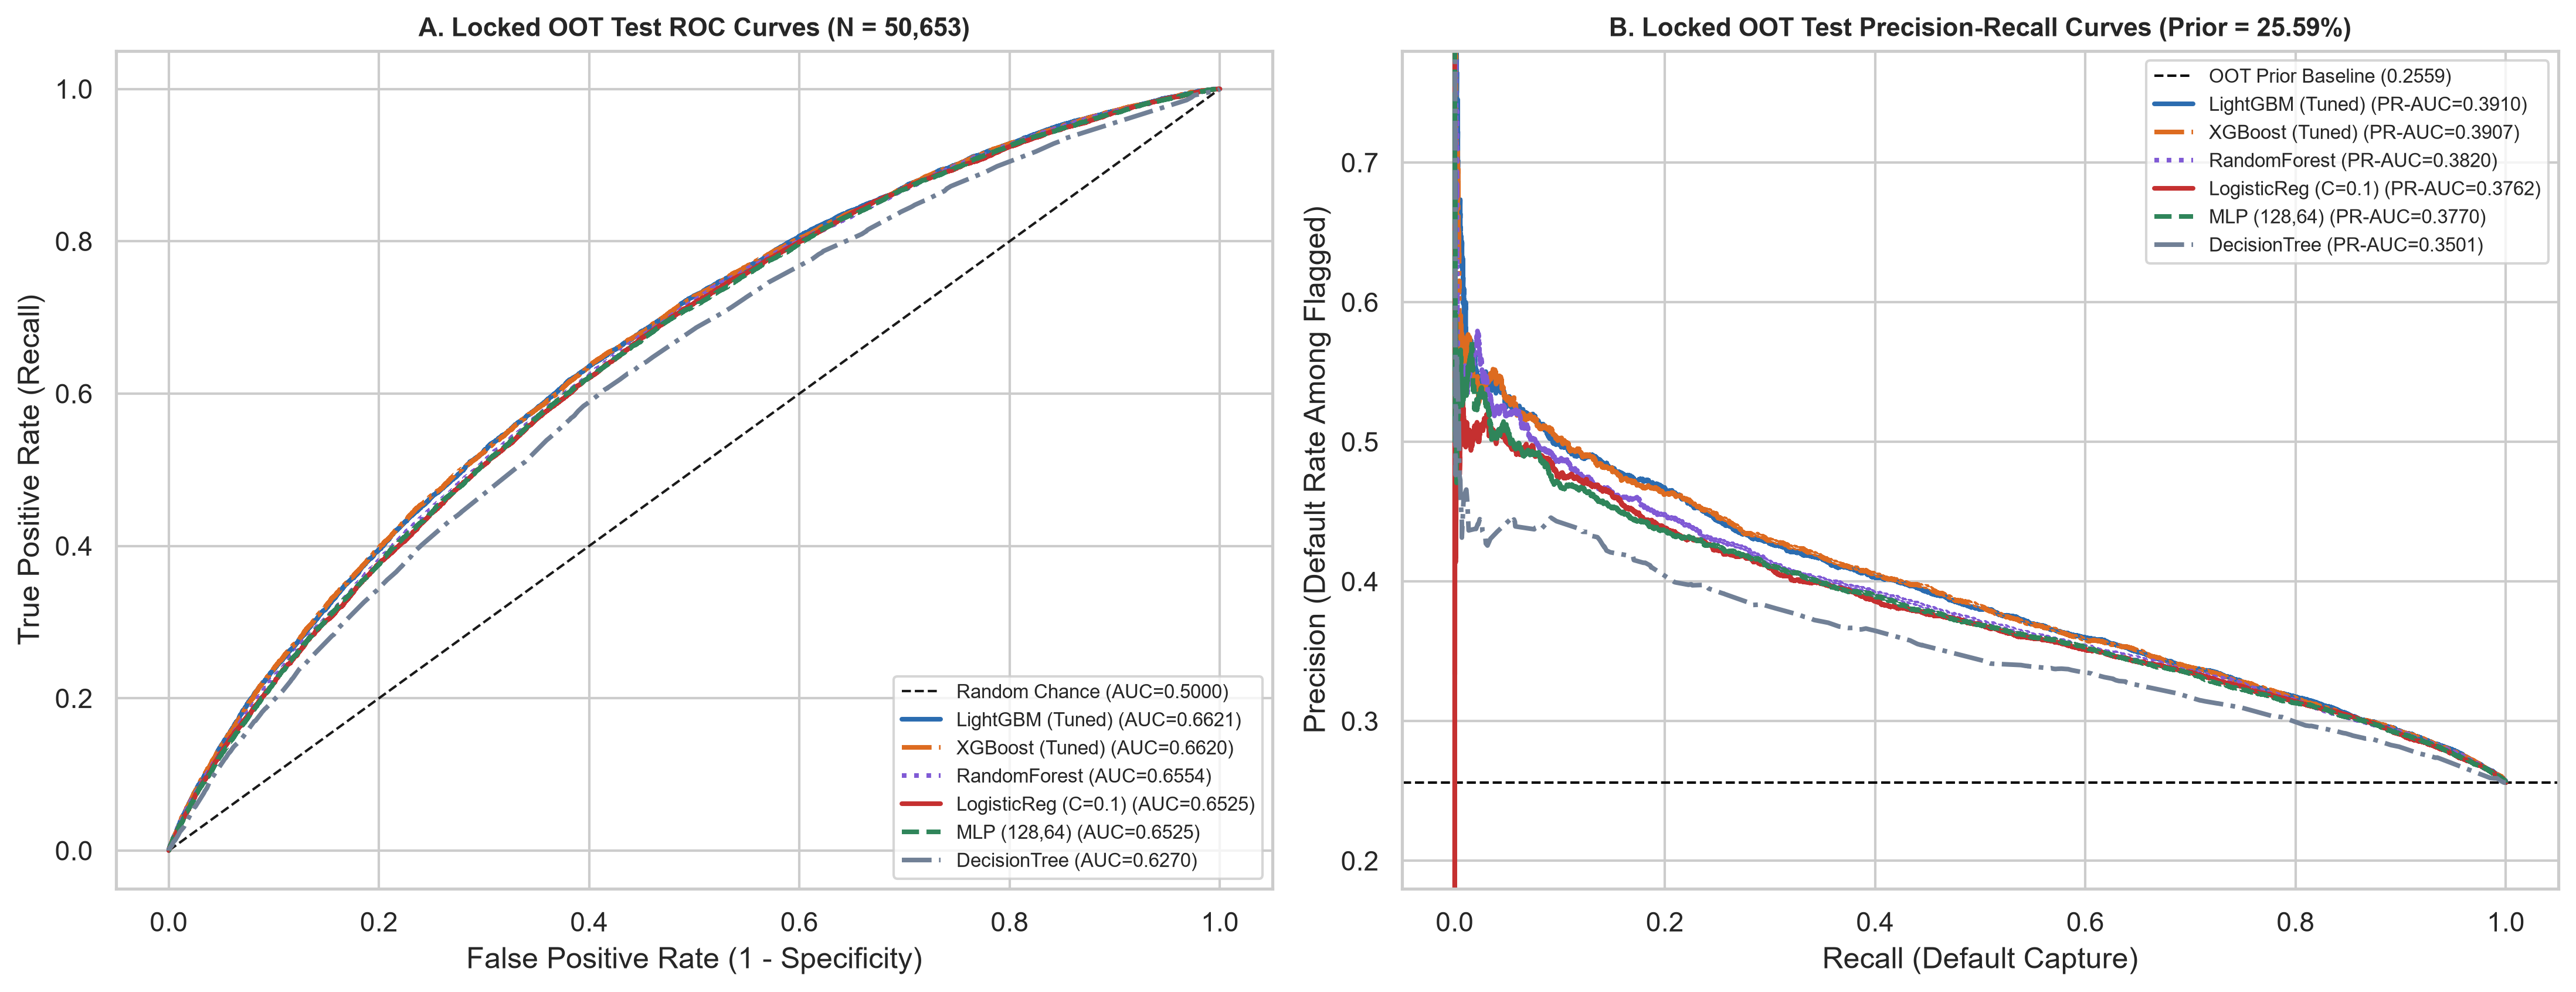
\includegraphics[width=0.95\textwidth]{figures/final_01_oot_roc_pr_curves.png}
  \caption{Out-of-Time ROC curves (left) and Precision--Recall curves relative to the $0.2559$ test baseline (right) on $N = 50{,}653$ contracts.}
  \label{fig:oot_roc_pr}
\end{figure}

Three clear findings stand out from Table~\ref{tab:oot_results}. First, the two tuned GBDT models lead all paradigms almost identically---\texttt{LightGBM} ($\text{OOT AUC} = 0.6621$, $\text{PR-AUC} = 0.3910$) and \texttt{XGBoost} ($0.6620$, $\text{PR-AUC} = 0.3907$)---achieving a $1.53\times$ Precision--Recall lift over the $0.2559$ test base rate. Second, both GBDTs clearly outperform \texttt{RandomForest} ($0.6554$, $-0.0067$ AUC), \texttt{LogisticRegression} ($0.6525$, $-0.0096$ AUC), the \texttt{MLP} baseline ($0.6525$), and the single \texttt{DecisionTree} ($0.6270$). Third, consistent with tabular benchmarks~\cite{gunnarsson2021,grinsztajn2022}, the controlled \texttt{MLP} baseline ($0.6525$, Brier $0.1834$, ECE $0.0573$) offers no ranking advantage over \texttt{LogisticRegression} ($0.6525$, ECE $0.0490$) while running $4.4\times$ slower ($7.5\text{ s}$ vs.\ $1.7\text{ s}$) and exhibiting weaker calibration. \texttt{LightGBM} is therefore selected as the primary champion model due to top OOT ranking, fast training time ($10.9\text{ s}$), strong Development probability calibration ($\text{ECE} = 0.0017$), and exact millisecond TreeSHAP attribution.

\subsection{Impact of Feature Engineering and Validation Strategy}
To evaluate how engineered features transfer to future contracts and how random train-test splitting distorts evaluation, Table~\ref{tab:fe_and_split} compares feature tiers on OOT Test alongside Stratified Random $80/20$ versus Locked OOT validation, illustrated visually in Figure~\ref{fig:rq3_split}.

\begin{table}[htbp]
  \centering
  \caption{Feature engineering ablation across tiers (Panel A) and Random 80/20 vs.\ Locked OOT validation bias (Panel B).}
  \label{tab:fe_and_split}
  \scriptsize
  \setlength{\tabcolsep}{3.0pt}
  \begin{tabular}{@{}llccccc@{}}
    \toprule
    \multicolumn{7}{@{}l}{\textbf{Panel A: Feature Tier Ablation on Locked OOT Test (ROC-AUC, $N = 50{,}653$)}} \\
    \midrule
    \textbf{Tier} & \textbf{Feature Additions} & \textbf{\texttt{LR}} & \textbf{\texttt{LGBM}} & \textbf{\texttt{XGB}} & \textbf{Avg.\ Gain vs.\ \texttt{F0}} & \\
    \midrule
    \texttt{F0} & Cleaned raw + 3 parsed fields & $0.6319$ & $0.6483$ & $0.6478$ & --- & \\
    \texttt{F1} & $+$29 domain ratios \& bureau split & $0.6345$ & $0.6506$ & $0.6500$ & $+0.0023$ & \\
    \textbf{\texttt{F2\_safe}} & \textbf{$+$ \texttt{branch}, \texttt{supplier}, \texttt{pincode}} & $\mathbf{0.6525}$ & $\mathbf{0.6621}$ & $\mathbf{0.6620}$ & $\mathbf{+0.0162}$ & \\
    \texttt{F2\_plus\_emp} & $+$ \texttt{Employee\_code\_ID} & $0.6543$ & $0.6636$ & $0.6635$ & $+0.0178$ & \\
    \midrule
    \multicolumn{7}{@{}l}{\textbf{Panel B: Stratified Random 80/20 vs.\ Locked OOT Validation on \texttt{F2\_safe}}} \\
    \midrule
    \textbf{Model} & \textbf{Rand.\ AUC} & \textbf{OOT AUC} & \textbf{Opt.\ Bias} & \textbf{Rand.\ ECE} & \textbf{OOT ECE} & \textbf{ECE Infl.} \\
    \midrule
    \texttt{LightGBM} (Tuned) & $0.6713$ & $\mathbf{0.6621}$ & $+0.0091$ & $\mathbf{0.0016}$ & $0.0491$ & $+0.0475$ ($30\times$) \\
    \texttt{XGBoost} (Tuned) & $\mathbf{0.6717}$ & $0.6620$ & $+0.0097$ & $0.0026$ & $\mathbf{0.0489}$ & $+0.0463$ ($19\times$) \\
    \texttt{RandomForest} (Base) & $0.6660$ & $0.6554$ & $+0.0106$ & $0.0128$ & $0.0499$ & $+0.0371$ ($4\times$) \\
    \texttt{LogisticReg.} ($C=0.1$) & $0.6629$ & $0.6525$ & $+0.0103$ & $0.0068$ & $0.0490$ & $+0.0421$ ($7\times$) \\
    \bottomrule
  \end{tabular}
\end{table}

\begin{figure}[htbp]
  \centering
  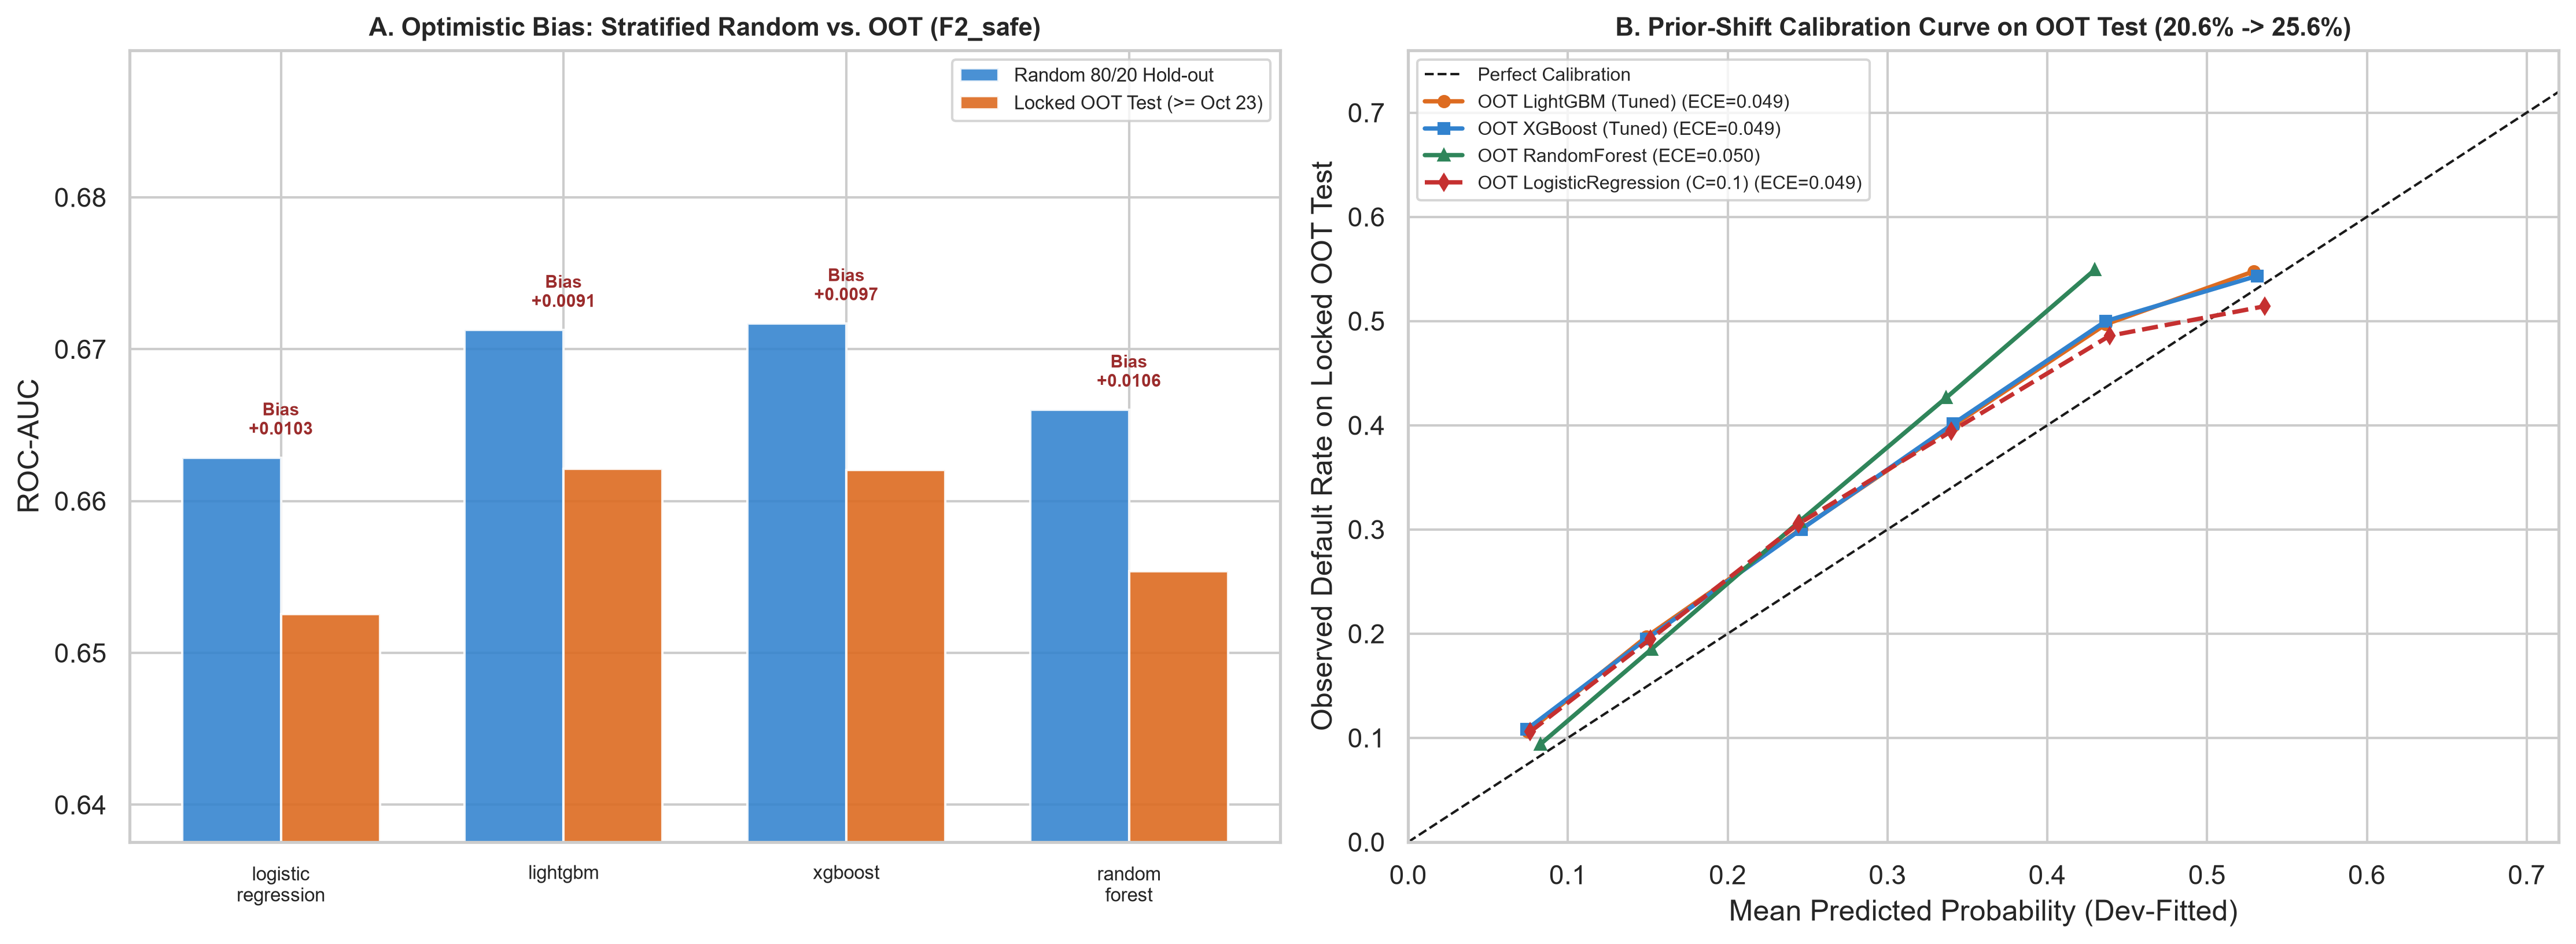
\includegraphics[width=0.95\textwidth]{figures/final_02_oot_vs_random_rq3.png}
  \caption{Comparison of Stratified Random splitting vs.\ Locked OOT Test: ROC-AUC optimism bias (left) and calibration curve shift caused by higher late-October default rates (right).}
  \label{fig:rq3_split}
\end{figure}

In Panel~A, domain financial engineering (\texttt{F0 -> F1}) delivers steady gains across all models ($+0.0021\text{--}+0.0026$ AUC), confirming the value of isolating non-scored bureau codes ($<300$) and adding leverage ratios. Introducing fold-safe OOF target encoding for dealer, branch, and postal channels (\texttt{F1 -> F2\_safe}) yields the largest leap ($+0.0115\text{--}+0.0180$ AUC) despite entity cold-start rates of $0.00\%$ on \texttt{branch\_id}, $0.80\%$ on \texttt{supplier\_id}, and $0.85\%$ on \texttt{Current\_pincode\_ID}. Adding \texttt{Employee\_code\_ID} (\texttt{F2\_plus\_emp}) adds $+0.0015$ short-term AUC over the 9-day October test window, yet suffers the highest unseen cold-start rate ($0.99\%$) and staff-turnover sensitivity, making \texttt{F2\_safe} safer for deployment.

Panel~B exposes two critical validation traps in standard random splitting. First, 80/20 Stratified Random evaluation artificially inflates ROC-AUC by $+0.0091$ to $+0.0106$ because uniform sampling shares same-day promotional cohorts and dealer clusters across train and test. Second, Random splitting reports nearly perfect probability calibration for LightGBM ($\text{ECE} = 0.0016$), hiding a $30$-fold ECE jump ($0.0491$) when default prevalence climbs from $20.63\%$ to $25.59\%$. As Figure~\ref{fig:rq3_split} (right) shows, every model's OOT reliability curve shifts parallel and roughly $5\text{ percentage points}$ above the diagonal, underscoring the need for temporal testing and periodic base-rate recalibration.

\subsection{Class Imbalance and Decision Threshold Analysis}
Table~\ref{tab:imbalance_thresh} evaluates six fold-isolated class-imbalance treatments (Panel~A) and five Development-frozen decision thresholds (Panel~B) on Stage-2 \texttt{LightGBM}. Figures~\ref{fig:imbalance_ablation} and~\ref{fig:thresholds} visualize the feature-ablation/imbalance contrast and the probability threshold trade-offs.

\begin{table}[htbp]
  \centering
  \caption{Imbalance correction strategies (Panel A) and Dev-frozen threshold transfer (Panel B) for Stage-2 \texttt{LightGBM} on Locked OOT Test ($N = 50{,}653$).}
  \label{tab:imbalance_thresh}
  \scriptsize
  \setlength{\tabcolsep}{3.5pt}
  \begin{tabular}{@{}lcccccc@{}}
    \toprule
    \multicolumn{7}{@{}l}{\textbf{Panel A: Fold-Isolated Imbalance Treatments on Locked OOT Test}} \\
    \midrule
    \textbf{Strategy} & \textbf{Train $N$} & \textbf{ROC-AUC} & \textbf{PR-AUC} & \textbf{Brier} & \textbf{ECE} & \textbf{Fit (s)} \\
    \midrule
    \textbf{\texttt{natural} ($\text{weight}=1.0$)} & $182{,}501$ & $0.6621$ & $0.3910$ & $\mathbf{0.1810}$ & $0.0491$ & $10.2$ \\
    \texttt{mild\_weight\_2.0} & $182{,}501$ & $\mathbf{0.6623}$ & $\mathbf{0.3912}$ & $0.1845$ & $0.0729$ & $10.7$ \\
    \texttt{class\_weight} ($\approx 3.85$) & $182{,}501$ & $0.6620$ & $0.3909$ & $0.2257$ & $\mathbf{0.2111}$ & $10.0$ \\
    \texttt{RUS 0.5} & $112{,}947$ & $0.6613$ & $0.3897$ & $0.1839$ & $0.0676$ & $\mathbf{7.3}$ \\
    \texttt{SMOTE 0.5} & $217{,}278$ & $0.6446$ & $0.3612$ & $0.1843$ & $0.0372$ & $18.1$ \\
    \texttt{SMOTE 1.0} & $289{,}704$ & $0.6252$ & $0.3453$ & $0.2013$ & $0.0977$ & $22.3$ \\
    \midrule
    \multicolumn{7}{@{}l}{\textbf{Panel B: Transfer of Pre-Frozen Operating Thresholds onto Locked OOT Test}} \\
    \midrule
    \textbf{Policy ($\tau_{\text{Dev}}$)} & \textbf{Flagged (\%)} & \textbf{Appr.\ (\%)} & \textbf{Prec.\ (\%)} & \textbf{Recall (\%)} & \textbf{F1-Score} & \textbf{Amt Loss (\%)} \\
    \midrule
    \texttt{Default} ($\tau = 0.500$) & $0.64$ & $99.36$ & $\mathbf{56.5}$ & $1.4$ & $0.0274$ & $13.12$ \\
    \texttt{Capacity Top-20\%} ($0.293$) & $20.18$ & $79.82$ & $42.0$ & $33.1$ & $0.3700$ & $9.95$ \\
    \texttt{Bayes 3:1} ($0.250$) & $31.38$ & $68.62$ & $38.6$ & $47.4$ & $0.4255$ & $8.78$ \\
    \texttt{F1-Optimal} ($0.205$) & $45.97$ & $54.03$ & $35.3$ & $63.5$ & $0.4540$ & $7.69$ \\
    \textbf{\texttt{Bayes 5:1} ($0.167$)} & $59.39$ & $40.61$ & $32.6$ & $\mathbf{75.6}$ & $\mathbf{0.4555}$ & $\mathbf{7.13}$ \\
    \bottomrule
  \end{tabular}
\end{table}

\begin{figure}[htbp]
  \centering
  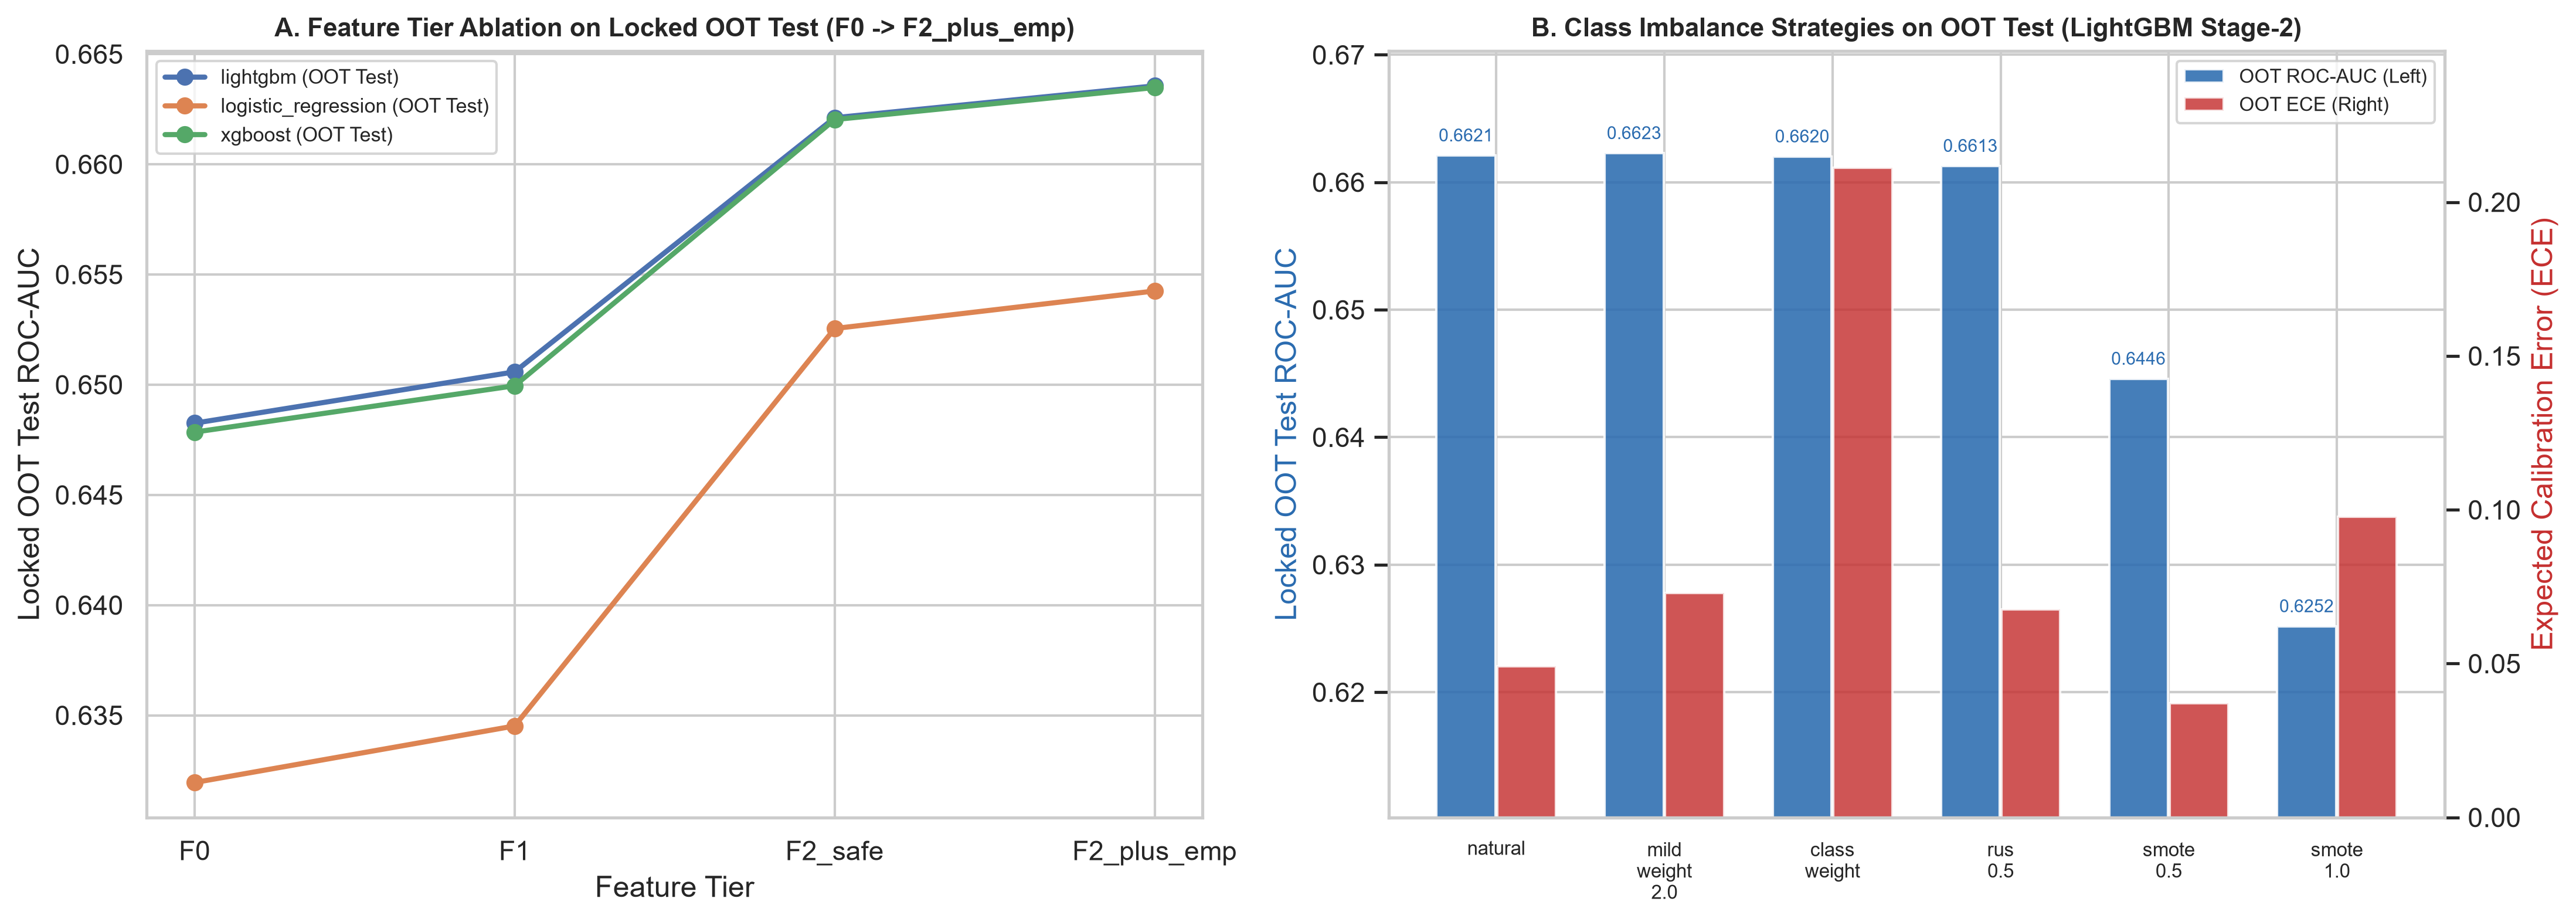
\includegraphics[width=0.95\textwidth]{figures/final_03_rq2_ablation_oot_and_imbalance.png}
  \caption{Out-of-Time feature tier progression (left) and fold-isolated imbalance performance confirming sharp SMOTE degradation on LightGBM (right).}
  \label{fig:imbalance_ablation}
\end{figure}

\begin{figure}[htbp]
  \centering
  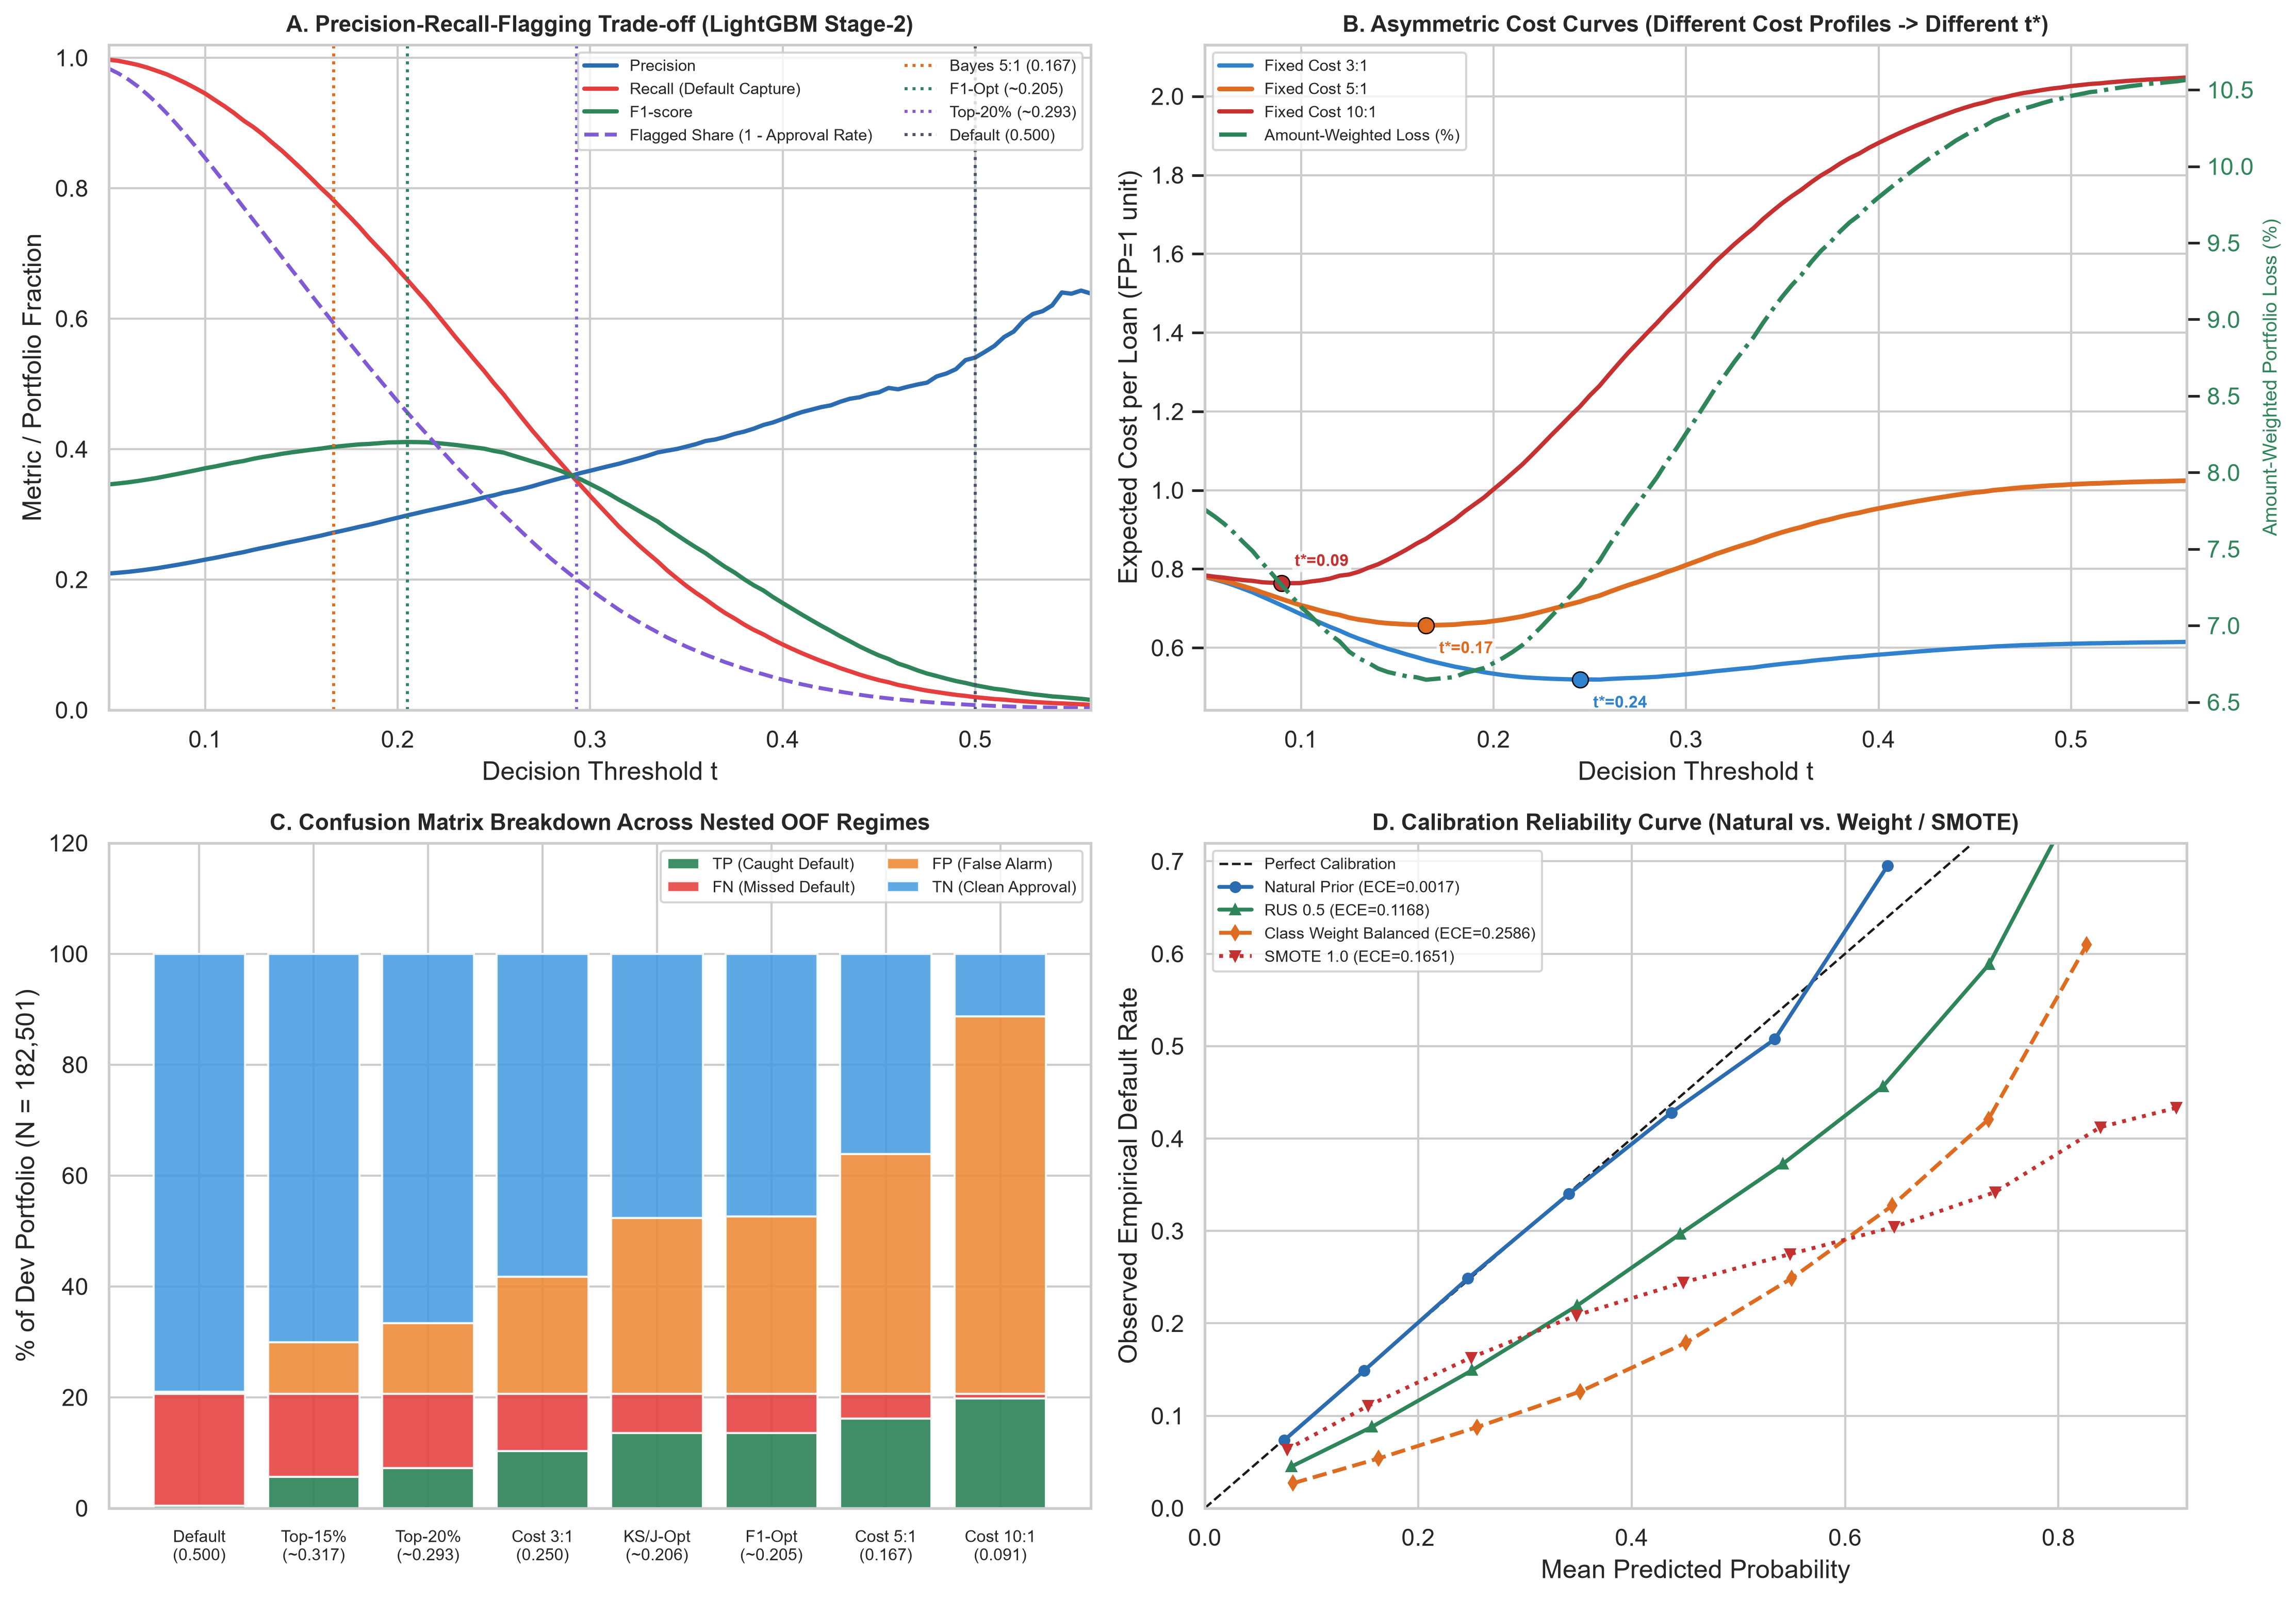
\includegraphics[width=0.95\textwidth]{figures/opt_01_threshold_tradeoffs.png}
  \caption{Threshold policy trade-offs across approval rate, recall, precision, portfolio financial loss, and calibration curves evaluated via nested 5-fold Development OOF.}
  \label{fig:thresholds}
\end{figure}

Three practical lessons emerge clearly. First, \textbf{strictly fold-isolated SMOTE actively harms GBDTs}: at ratio $1.0$, \texttt{SMOTE} drops LightGBM OOT ROC-AUC by $-0.0369$ ($0.6621 \to 0.6252$) and PR-AUC by $-0.0456$. This happens because linear Euclidean interpolation across a $123$-column matrix containing dozens of binary KYC flags and one-hot categories creates unrealistic fractional synthetic points between $0$ and $1$, causing trees to overfit artificial split boundaries. Notably, \texttt{SMOTE 0.5} exhibits a lower raw OOT ECE ($0.0372$) than \texttt{natural} ($0.0491$) only because SMOTE's upward probability inflation (Dev ECE $0.0866$ vs.\ $0.0017$ for \texttt{natural}) accidentally cancels part of the $+4.96\text{ percentage-point}$ late-October prior shift, while still degrading ROC-AUC ($-0.0175$) and Brier score ($0.1843$ vs.\ $0.1810$). Second, heavy balanced weighting (\texttt{class\_weight}) does not improve ROC-AUC ($0.6620$) while quadrupling calibration error ($\text{ECE} = 0.2111$), confirming~\cite{goorbergh2022}: training on natural priors achieves the best Brier score ($0.1810$) without distorting risk scores.

Third, \textbf{threshold tuning dramatically cuts financial loss}. Relying on the standard cutoff $\tau = 0.500$ flags only $0.64\%$ of loans, misses $98.6\%$ of all defaults, and incurs $13.12\%$ principal-weighted loss. Lowering the cutoff to Bayesian cost-aligned levels cuts expected loss nearly in half ($7.13\%$ at $\tau = 0.167$, capturing $75.6\%$ of defaults; $8.78\%$ at $\tau = 0.250$ while retaining $68.6\%$ direct approvals), with OOT flagging volumes matching Development forecasts within $\pm 0.36\text{ percentage points}$. Risk ranking across predicted probability deciles is strictly monotonic: observed OOT default rates rise $5.04\times$ from $9.36\%$ in the safest decile (\texttt{D1}) to $47.21\%$ in the highest-risk decile (\texttt{D10}).

\subsection{Model Explainability (SHAP) and Practical Policy}
To verify how predictions are generated and audit model fairness, Figure~\ref{fig:shap_global} presents global TreeSHAP feature attributions on unseen Development Fold~4, while Figure~\ref{fig:shap_cases} tracks feature rank stability onto the Locked OOT Test cohort alongside four concrete loan decisions. Exact LightGBM TreeSHAP log-odds additivity holds to floating-point machine precision (error $1.47\times 10^{-14}$ on OOT Test), and global importance rankings are remarkably consistent both across GBDT architectures (\texttt{LightGBM} vs.\ \texttt{XGBoost} Spearman $\rho = 0.974$) and across time (Development vs.\ OOT Test $\rho = 0.973$). Note that SHAP values reflect predictive correlations learned from historical contracts rather than causal effects.

\begin{figure}[htbp]
  \centering
  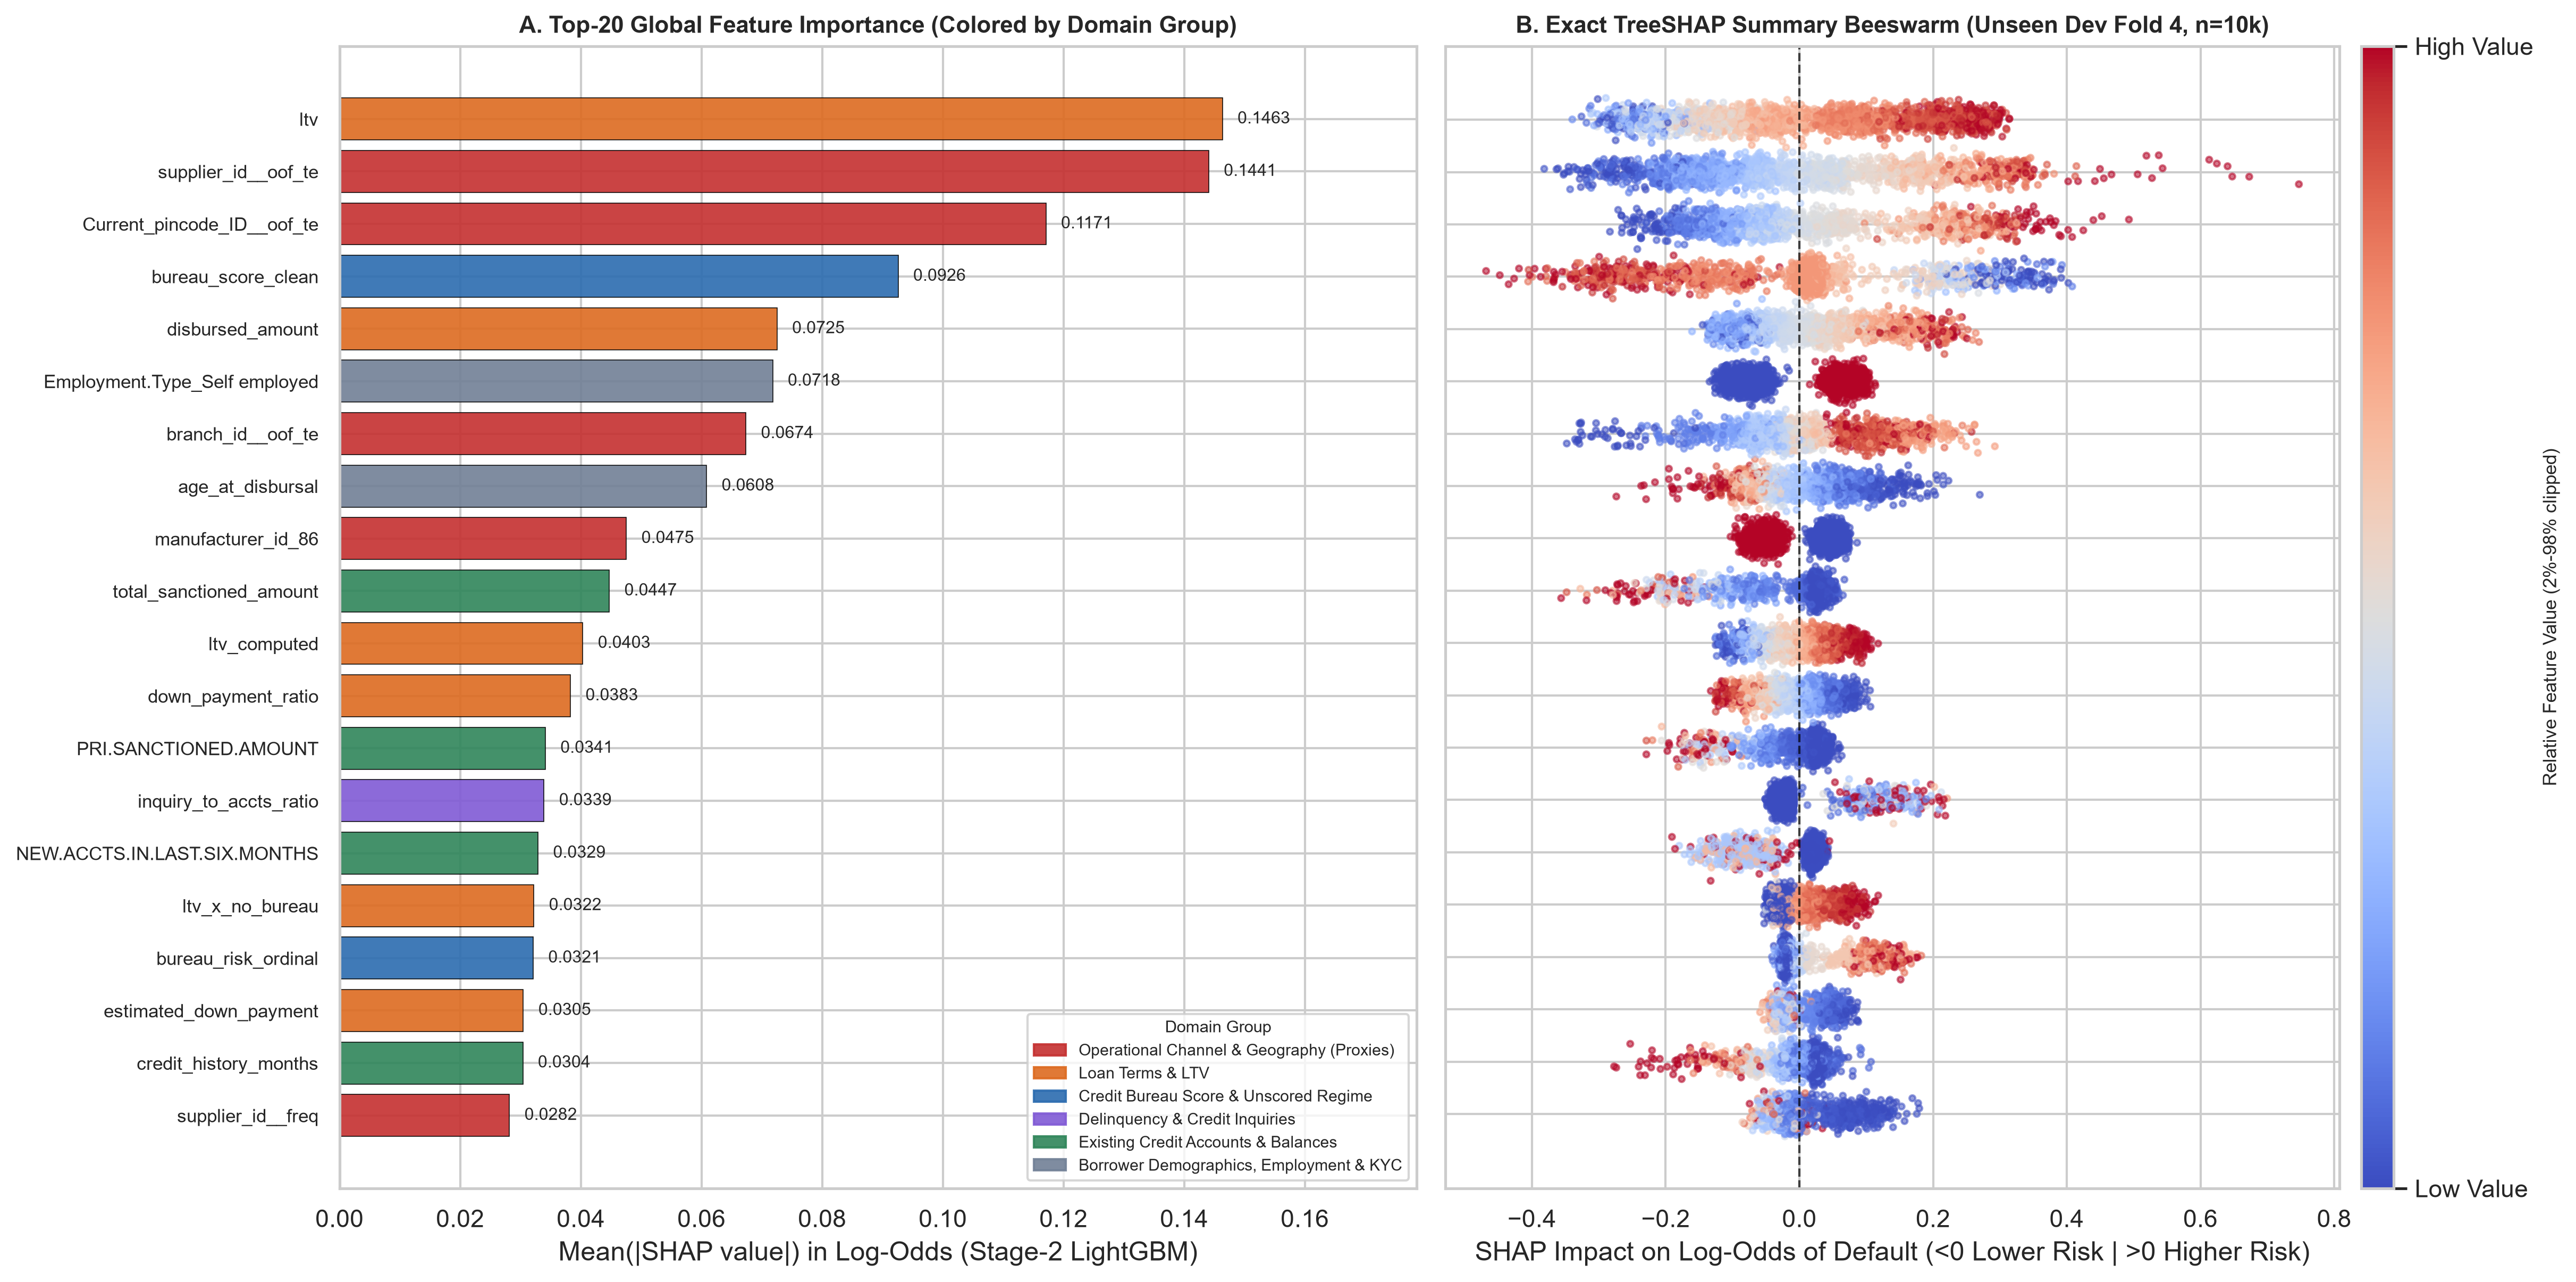
\includegraphics[width=0.95\textwidth]{figures/exp_01_shap_global_and_beeswarm.png}
  \caption{Top-20 global features ranked by mean $|\text{SHAP}|$ (left) and TreeSHAP beeswarm plot showing how high/low values shift default log-odds (right).}
  \label{fig:shap_global}
\end{figure}

Across the portfolio, operational channels and geography (\texttt{supplier\_id}, \texttt{branch\_id}, vehicle make, and \texttt{Current\_pincode\_ID}) account for $28.90\%$ of total OOT SHAP weight, followed by loan terms and LTV ($23.81\%$), existing credit accounts, recent openings, and balances ($19.39\%$), borrower demographics, employment, and KYC ($12.58\%$), delinquency history and inquiries ($7.76\%$), and numerical bureau scores ($7.55\%$). Key individual risk drivers align with domain finance intuition: higher \texttt{ltv} (especially above $75\%$), high-risk dealerships (\texttt{supplier\_id\_\_oof\_te}), weaker \texttt{bureau\_score\_clean} ($<620$), larger \texttt{disbursed\_amount}, \texttt{Self employed} status, younger borrower age, and recent credit inquiries all increase default risk. Exact pairwise SHAP analysis on XGBoost further confirms strong non-linear interactions between \texttt{disbursed\_amount} $\times$ \texttt{ltv} and between \texttt{ltv} $\times$ dealership/bureau scores.

\begin{figure}[htbp]
  \centering
  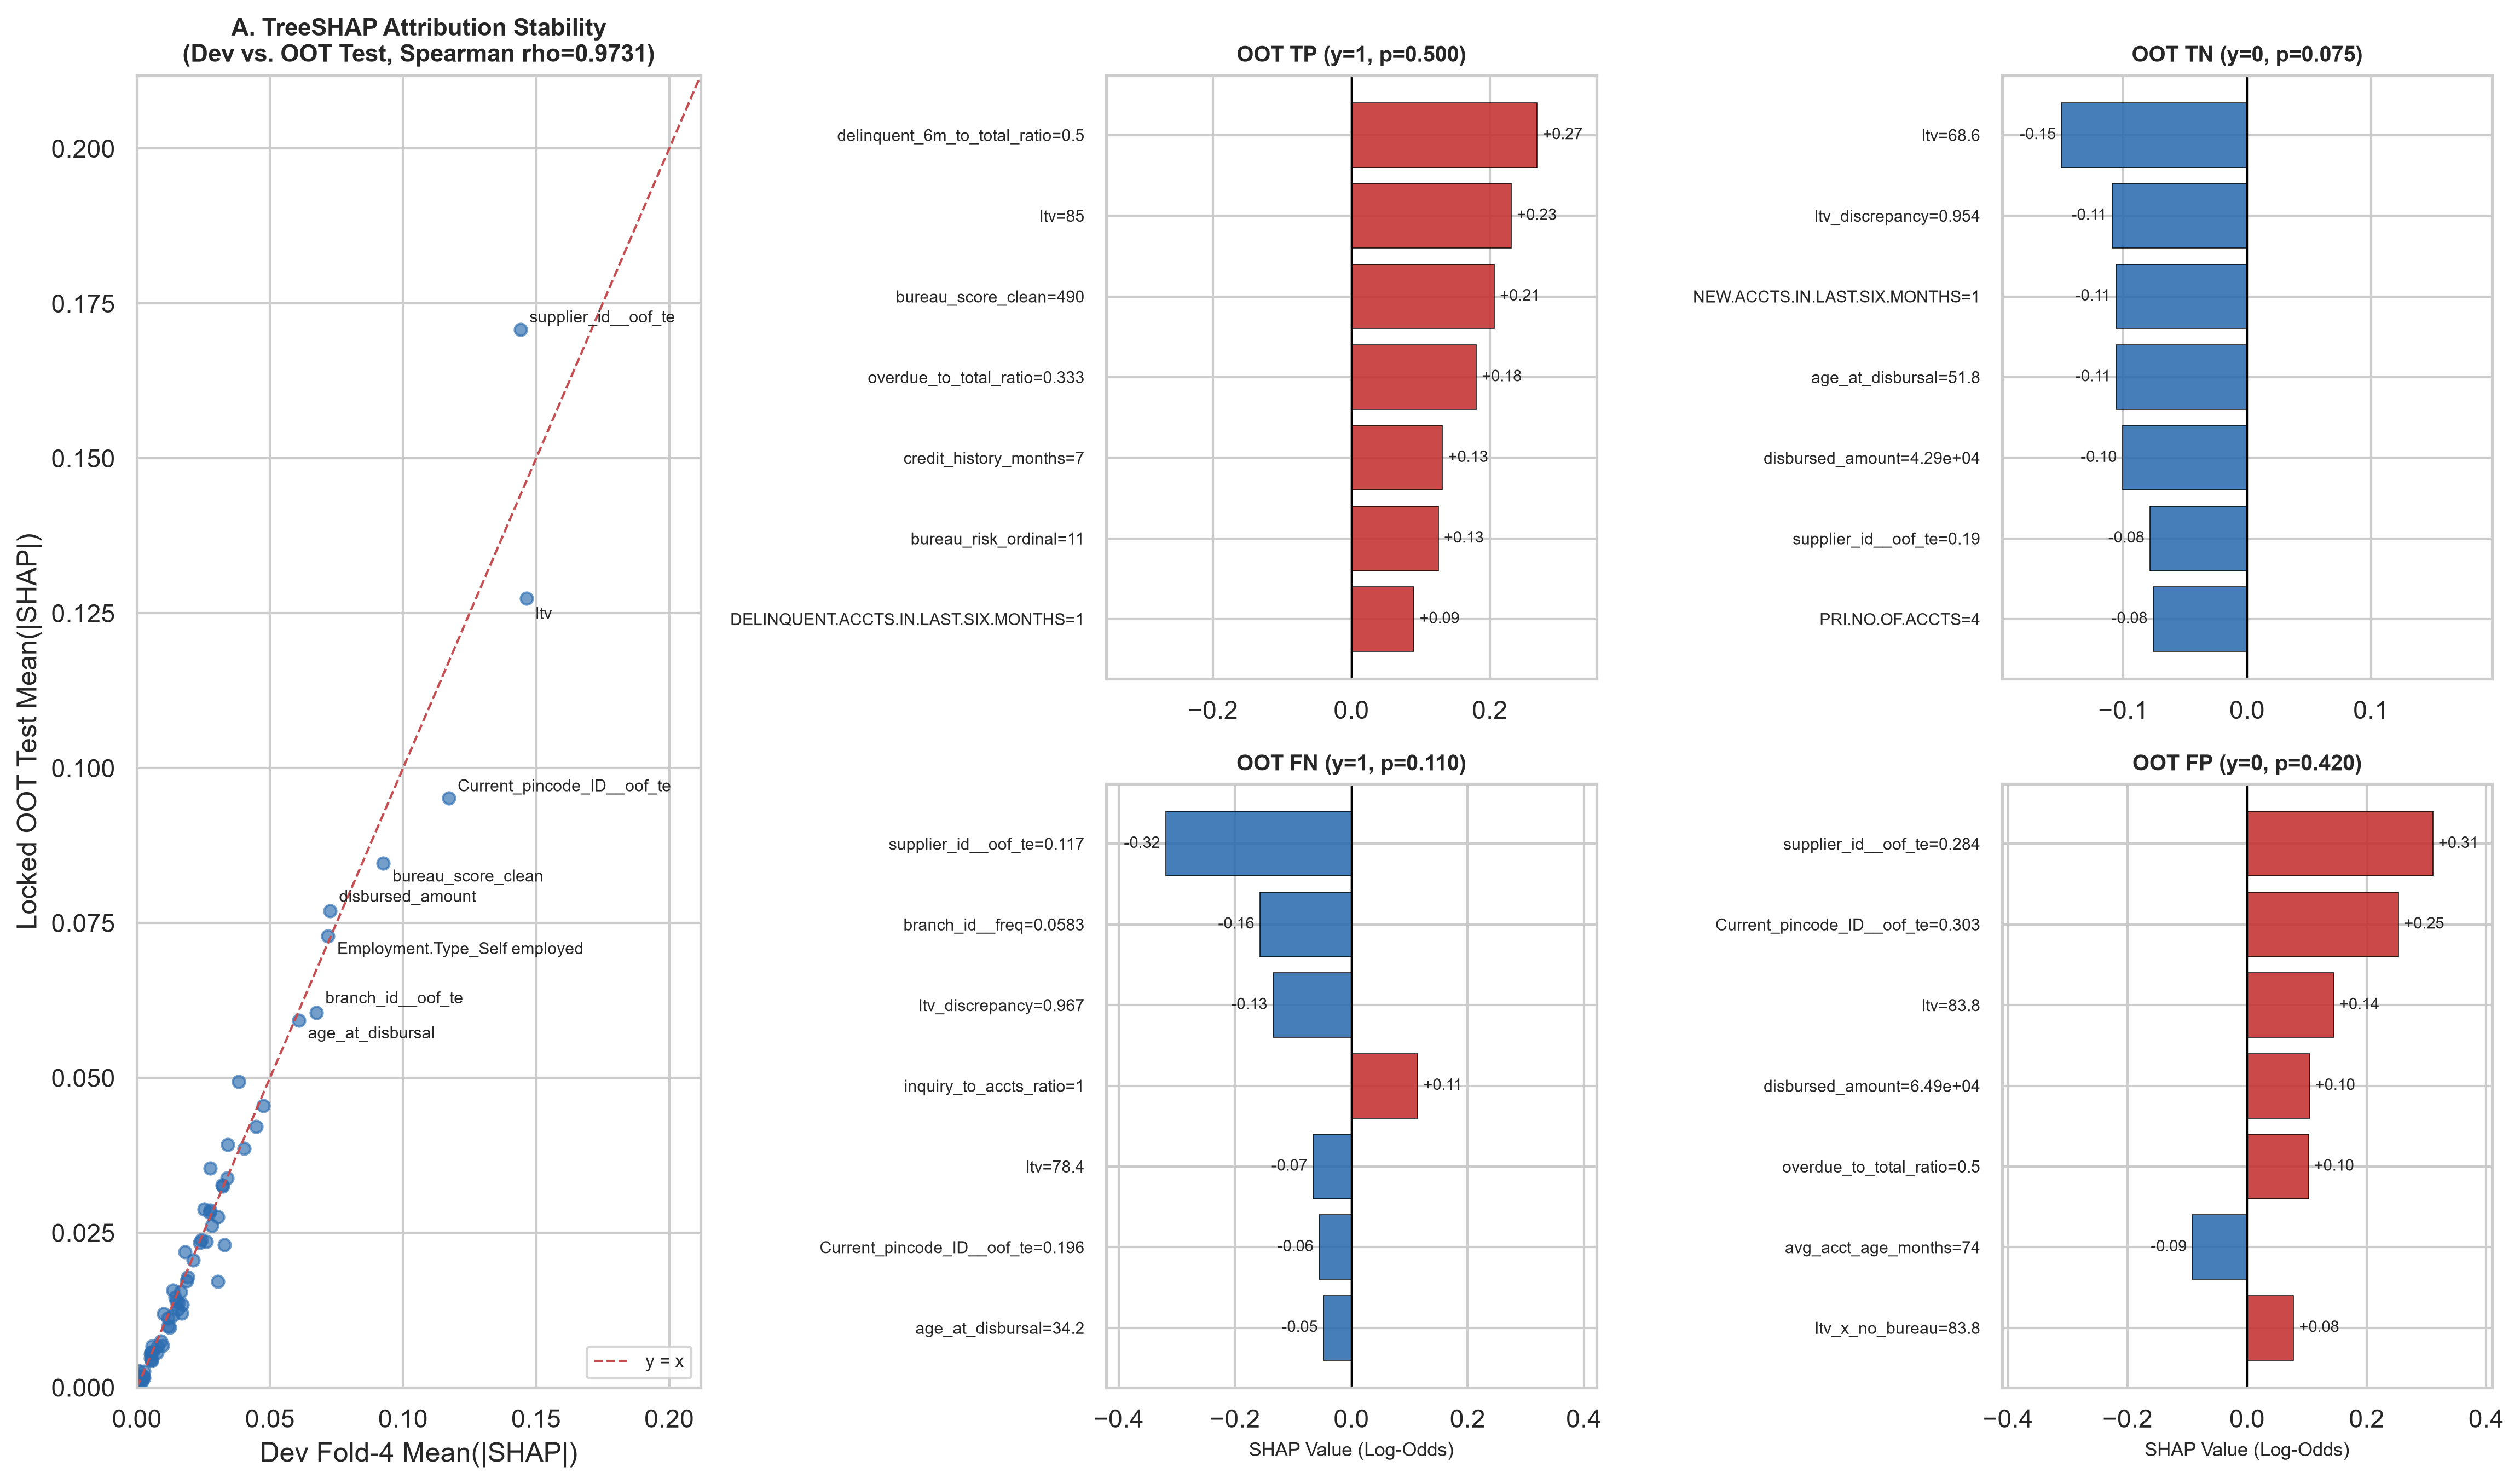
\includegraphics[width=0.95\textwidth]{figures/final_05_test_xai_stability_and_errors.png}
  \caption{Cross-time TreeSHAP importance stability between Development and OOT Test ($\rho = 0.973$, left) and four individual OOT explanation case studies (right).}
  \label{fig:shap_cases}
\end{figure}

Inspecting individual OOT cases (Figure~\ref{fig:shap_cases}, right) and subgroup cohorts reveals important operational nuances:
\begin{itemize}
  \item \textbf{Clear Successes (\texttt{TP 630094}, $\hat{p}=0.500$; \texttt{TN 645014}, $\hat{p}=0.075$):} The high-risk default case combines $85\%$ LTV, bureau score $490$, and recent 6-month delinquency, whereas the safe case pairs low leverage ($68.6\%$ LTV), solid credit score ($680$), and borrower maturity ($51.8$ years).
  \item \textbf{Thin-File Blind Spot (\texttt{FN 621929}, $y=1$, $\hat{p}=0.110$ vs.\ \texttt{FP 652048}, $y=0$, $\hat{p}=0.420$):} When an applicant has no bureau score ($0$), strong dealership/pincode priors heavily sway predictions---letting a risky thin-file loan slip past at a safe dealership (\texttt{supplier TE = 0.117}) while flagging a borrower who ultimately repaid (\texttt{FP 652048}) due to combined high dealership/pincode risk (\texttt{supplier TE = 0.284}, \texttt{pincode TE = 0.303}), $83.8\%$ LTV, and an overdue secondary guarantor account (\texttt{overdue\_to\_total\_ratio = 0.50}).
  \item \textbf{Subgroup Separation Gap:} Across OOT Test slices, LightGBM separates risk much better for borrowers with credit bureau scores ($\text{AUC} = 0.683$) than for unscored thin-file borrowers ($\text{AUC} = 0.645$, $-3.8\text{ percentage points}$), and performs stronger on mature borrowers aged $46+$ ($\text{AUC} = 0.694$) than ages $18\text{--}25$ ($\text{AUC} = 0.642$).
\end{itemize}

Because $59\%$ flagging is too broad for blanket automatic rejections and dealer proxies carry nearly $29\%$ SHAP weight, the champion model should operate inside a \textbf{Three-Tier Human-in-the-Loop Underwriting Policy}: (1) \textbf{Auto-Approve} ($\hat{p} < 0.167$, $\sim 41\%$ volume), adding an income-verification rule if a thin-file borrower seeks $>78\%$ LTV at a low-risk dealer; (2) \textbf{Manual Underwriting Review} ($0.167 \le \hat{p} < 0.317$, $\sim 44\%$ volume), where phone checks capture up to $75.6\%$ of defaults while protecting good applicants flagged by regional proxies; and (3) \textbf{Counter-Offer or Decline} ($\hat{p} \ge 0.317$, top $15\%$), requiring higher down payments supported by borrower-specific SHAP reason codes alongside periodic base-rate probability recalibration when seasonal risk shifts.

\section{Conclusion and Future Work}
\label{sec:conclusion}

In this project, we built and evaluated a leakage-free machine learning pipeline to predict First Payment Default across $233{,}154$ LTFS vehicle loans, yielding four main conclusions:

\begin{enumerate}[itemsep=1pt,topsep=2pt]
  \item \textbf{Gradient Boosting Leads Credit Risk Separation:} Tuned \texttt{LightGBM} ($\text{OOT AUC} = 0.6621$) and \texttt{XGBoost} ($0.6620$) achieve top performance and clearly outperform \texttt{RandomForest} ($0.6554$), \texttt{LogisticRegression} ($0.6525$), the controlled \texttt{MLP} baseline ($0.6525$), and \texttt{DecisionTree} ($0.6270$). \texttt{LightGBM} provides the best balance of training speed ($10.9\text{ s}$), Development calibration ($\text{ECE} = 0.0017$), and exact TreeSHAP explainability.
  \item \textbf{Domain Engineering and Channel Encoding Matter:} Separating non-scored credit bureau codes ($<300$) from numeric scores ($300\text{--}890$) and adding leverage/distress ratios improves OOT generalization across all models ($+0.0021$ to $+0.0026$ AUC), while leak-free Out-of-Fold Empirical-Bayes target encoding on dealer, branch, and postal channels contributes $+0.0115$ to $+0.0180$ AUC gain on future cohorts.
  \item \textbf{Time-Based Validation Prevents Optimism Bias:} Standard random 80/20 splitting overstates OOT ROC-AUC by $+0.0091$ to $+0.0106$ and conceals a $30$-fold calibration degradation ($\text{ECE } 0.0016 \to 0.0491$) triggered when late-October default prevalence jumps from $20.63\%$ to $25.59\%$.
  \item \textbf{Threshold Optimization Beats Synthetic Resampling:} Fold-isolated \texttt{SMOTE} degrades \texttt{LightGBM} OOT ROC-AUC down to $0.6252$, and heavy balanced class weighting distorts calibration ($\text{ECE} = 0.2111$). Training on natural empirical priors coupled with a Bayesian $5{:}1$ cost threshold ($\tau = 0.167$) preserves ranking while nearly halving principal-weighted portfolio loss compared to the naive $0.50$ cutoff ($7.13\%$ vs.\ $13.12\%$).
\end{enumerate}

\subsection{Limitations and Future Work}
Four methodological and data boundaries should be considered when deploying these findings. First, the labeled corpus spans three months (August--October 2018) and omits borrower income, debt-to-income ratios, loan tenure, and vehicle depreciation, creating an observable information ceiling near $\text{OOT AUC} \approx 0.662$ ($0.645$ on thin-file loans); incorporating alternative cashflow or utility signals could narrow this gap. Second, the neural \texttt{MLP} was evaluated as a controlled baseline architecture without exhaustive Optuna hyperparameter tuning or learned entity embeddings, so deeper tabular architectures could be revisited under equalized tuning budgets. Third, nearly $29\%$ of OOT SHAP attribution stems from dealer and postal proxies, motivating fair-lending constraints and rolling target-encoding refreshes as channels evolve. Finally, production deployment should incorporate online log-odds intercept recalibration for seasonal prior shifts and reject-inference auditing across multi-quarter horizons.


\clearpage
\phantomsection
\addcontentsline{toc}{section}{References}
{\raggedright
\begin{thebibliography}{99}

\bibitem{ltfs2019}
L\&T Financial Services (LTFS), ``LTFS Data Science FinHack: Vehicle Loan Default Prediction Dataset,'' Kaggle public archive (\texttt{mamtadhaker/lt-vehicle-loan-default-prediction}), 2019. [Online]. Available: \url{https://www.kaggle.com/datasets/mamtadhaker/lt-vehicle-loan-default-prediction}

\bibitem{agarwal2008}
S.~Agarwal, B.~W. Ambrose, and S.~Chomsisengphet, ``Determinants of automobile loan default and prepayment,'' \textit{Economic Perspectives}, Federal Reserve Bank of Chicago, vol.~32, no.~3, pp.~17--28, 2008. [Online]. Available: \url{https://www.chicagofed.org/publications/economic-perspectives/2008/3qtr2008-part2-agarwal-et-al}

\bibitem{baesens2003}
B.~Baesens, T.~Van Gestel, S.~Viaene, M.~Stepanova, J.~A.~K. Suykens, and J.~Vanthienen, ``Benchmarking state-of-the-art classification algorithms for credit scoring,'' \textit{Journal of the Operational Research Society}, vol.~54, no.~6, pp.~627--635, 2003, doi: \url{https://doi.org/10.1057/palgrave.jors.2601545}.

\bibitem{lessmann2015}
S.~Lessmann, B.~Baesens, H.-V. Seow, and L.~C. Thomas, ``Benchmarking state-of-the-art classification algorithms for credit scoring: An update of research,'' \textit{European Journal of Operational Research}, vol.~247, no.~1, pp.~124--136, 2015, doi: \url{https://doi.org/10.1016/j.ejor.2015.05.030}.

\bibitem{breiman2001}
L.~Breiman, ``Random Forests,'' \textit{Machine Learning}, vol.~45, no.~1, pp.~5--32, 2001, doi: \url{https://doi.org/10.1023/A:1010933404324}.

\bibitem{chen2016}
T.~Chen and C.~Guestrin, ``XGBoost: A Scalable Tree Boosting System,'' in \textit{Proc.\ 22nd ACM SIGKDD Int.\ Conf.\ Knowledge Discovery and Data Mining (KDD '16)}, 2016, pp.~785--794, doi: \url{https://doi.org/10.1145/2939672.2939785}.

\bibitem{ke2017}
G.~Ke, Q.~Meng, T.~Finley, T.~Wang, W.~Chen, W.~Ma, Q.~Ye, and T.-Y. Liu, ``LightGBM: A Highly Efficient Gradient Boosting Decision Tree,'' in \textit{Advances in Neural Information Processing Systems 30 (NIPS 2017)}, 2017, pp.~3146--3154. [Online]. Available: \url{https://dl.acm.org/doi/10.5555/3294996.3295074}

\bibitem{gunnarsson2021}
B.~R. Gunnarsson, S.~vanden Broucke, B.~Baesens, M.~\'Oskarsd\'ottir, and W.~Lemahieu, ``Deep learning for credit scoring: Do or don't?'' \textit{European Journal of Operational Research}, vol.~295, no.~1, pp.~292--305, 2021, doi: \url{https://doi.org/10.1016/j.ejor.2021.03.006}.

\bibitem{grinsztajn2022}
L.~Grinsztajn, E.~Oyallon, and G.~Varoquaux, ``Why do tree-based models still outperform deep learning on typical tabular data?'' in \textit{Advances in Neural Information Processing Systems 35 (NeurIPS 2022)}, 2022, pp.~507--520. [Online]. Available: \url{https://arxiv.org/abs/2207.08815}

\bibitem{wu2025}
X.~Wu, ``Vehicle Loan Default Prediction Based on Machine Learning,'' \textit{Theoretical and Natural Science}, vol.~120, no.~1, pp.~209--220, 2025, doi: \url{https://doi.org/10.54254/2753-8818/2025.AD26291}.

\bibitem{chawla2002}
N.~V. Chawla, K.~W. Bowyer, L.~O. Hall, and W.~P. Kegelmeyer, ``SMOTE: Synthetic Minority Over-sampling Technique,'' \textit{Journal of Artificial Intelligence Research}, vol.~16, pp.~321--357, 2002, doi: \url{https://doi.org/10.1613/jair.953}.

\bibitem{goorbergh2022}
R.~van den Goorbergh, M.~van Smeden, D.~Timmerman, and B.~Van Calster, ``The harm of class imbalance corrections for risk prediction models: illustration and simulation using logistic regression,'' \textit{Journal of the American Medical Informatics Association (JAMIA)}, vol.~29, no.~9, pp.~1525--1534, 2022, doi: \url{https://doi.org/10.1093/jamia/ocac093}.

\bibitem{saito2015}
T.~Saito and M.~Rehmsmeier, ``The Precision-Recall Plot Is More Informative than the ROC Plot When Evaluating Binary Classifiers on Imbalanced Datasets,'' \textit{PLoS ONE}, vol.~10, no.~3, p.~e0118432, 2015, doi: \url{https://doi.org/10.1371/journal.pone.0118432}.

\bibitem{elkan2001}
C.~Elkan, ``The Foundations of Cost-Sensitive Learning,'' in \textit{Proc.\ 17th Int.\ Joint Conf.\ Artificial Intelligence (IJCAI '01)}, 2001, pp.~973--978. [Online]. Available: \url{https://www.ijcai.org/Proceedings/01/Papers/139.pdf}

\bibitem{bahnsen2014}
A.~C. Bahnsen, D.~Aouada, and B.~Ottersten, ``Example-Dependent Cost-Sensitive Logistic Regression for Credit Scoring,'' in \textit{Proc.\ 13th IEEE Int.\ Conf.\ Machine Learning and Applications (ICMLA)}, 2014, pp.~263--269, doi: \url{https://doi.org/10.1109/ICMLA.2014.48}.

\bibitem{lundberg2017}
S.~M. Lundberg and S.-I. Lee, ``A Unified Approach to Interpreting Model Predictions,'' in \textit{Advances in Neural Information Processing Systems 30 (NIPS 2017)}, 2017, pp.~4765--4774. [Online]. Available: \url{https://arxiv.org/abs/1705.07874}

\bibitem{lundberg2020}
S.~M. Lundberg, G.~Erion, H.~Chen, A.~DeGrave, J.~M. Prutkin, B.~Nair, R.~Katz, J.~Himmelfarb, N.~Bansal, and S.-I. Lee, ``From local explanations to global understanding with explainable AI for trees,'' \textit{Nature Machine Intelligence}, vol.~2, no.~1, pp.~56--67, 2020, doi: \url{https://doi.org/10.1038/s42256-019-0138-9}.

\bibitem{bussmann2021}
N.~Bussmann, P.~Giudici, D.~Marinelli, and J.~Papenbrock, ``Explainable Machine Learning in Credit Risk Management,'' \textit{Computational Economics}, vol.~57, no.~1, pp.~203--216, 2021, doi: \url{https://doi.org/10.1007/s10614-020-10042-0}.

\bibitem{miccibarreca2001}
D.~Micci-Barreca, ``A preprocessing scheme for high-cardinality categorical attributes in classification and prediction problems,'' \textit{ACM SIGKDD Explorations Newsletter}, vol.~3, no.~1, pp.~27--32, 2001, doi: \url{https://doi.org/10.1145/507533.507538}.

\bibitem{akiba2019}
T.~Akiba, S.~Sano, T.~Yanase, T.~Ohta, and M.~Koyama, ``Optuna: A Next-generation Hyperparameter Optimization Framework,'' in \textit{Proc.\ 25th ACM SIGKDD Int.\ Conf.\ Knowledge Discovery and Data Mining (KDD '19)}, 2019, pp.~2623--2631, doi: \url{https://doi.org/10.1145/3292500.3330701}.

\end{thebibliography}
}


\end{document}
